% (C) Marc Lijour, 2020 
% This course content for the Blockchain developer certificate at George Brown College 
% authored by Marc Lijour is licensed under CC BY-SA 4.0. 
% To view a copy of this license, visit https://creativecommons.org/licenses/by-sa/4.0
% ---
% Lecture 3: Institutional blockchain usecases in FinTech and other industries
% Addressed to the AFR cohort and the regular cohort, Fall 2020

\frame{
    \frametitle{Quick recap from lecture 1 and the first Quizz}
    \begin{alertblock}{About Academic Honesty/Dishonesty}
    \textbf{From the course outline:}
    ``The minimal consequence for submitting a plagiarized, purchased, contracted, or in any manner inappropriately negotiated or falsified assignment, test, essay, project, or any evaluated material will be a grade of zero on that material.\\
    To view George Brown College policies please go to \url{www.georgebrown.ca/policies}''
    \end{alertblock}
    Refresher on a few key points:
    \begin{itemize}
        \item The definition of money
        \item Representative vs Fiat money
        \item Multiple concurrent currencies are not a first in the history of money
        \item Gresham's law
        \item Will Bitcoin (or an altcoin) perdure?
        \item Central banks unconventional policies: why does it matter in 2020?
    \end{itemize}
}

% ======================================================================================================
%                         Value prop and market size
% ======================================================================================================
\section{Business potential}

%----------------------------------------------------------------------------
\subsection{Market size}

\frame{
    \frametitle{Top industries and blockchain use-cases}
    \begin{block}{According to \citeauthor{idc2018:spendingforecast} (\citeyear{idc2018:spendingforecast})}
        \begin{itemize}
            \item financial sector (\$552 million in 2018) --custody and asset tracking, trade finance, in addition to cross-border payments and settlements
            \item distribution and services sector (\$379 million in 2018) --asset/goods management and lot lineage/provenance
            \item manufacturing and resources sector (\$334 million in 2018) --as above
        \end{itemize}
    \end{block}
}

\frame{
    \frametitle{Market size for blockchain applications}
	\begin{figure}
		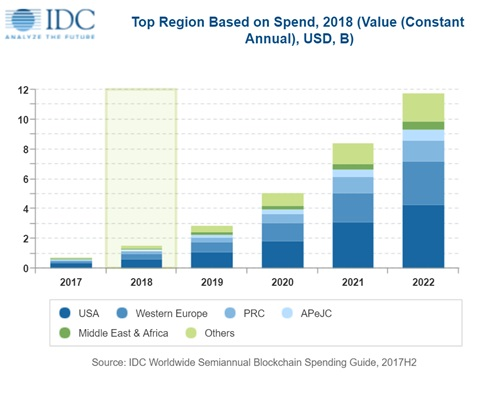
\includegraphics[height=6cm]{../pics/blockchain/idc2018-spendingforecast}
    \caption{from \citeauthor{idc2018:spendingforecast} (\citeyear{idc2018:spendingforecast})}
	\end{figure}
}

%----------------------------------------------------------------------------
\subsection{Value proposition by industry}

\frame{
	\frametitle{Top advantages per industry}
	\begin{figure}
		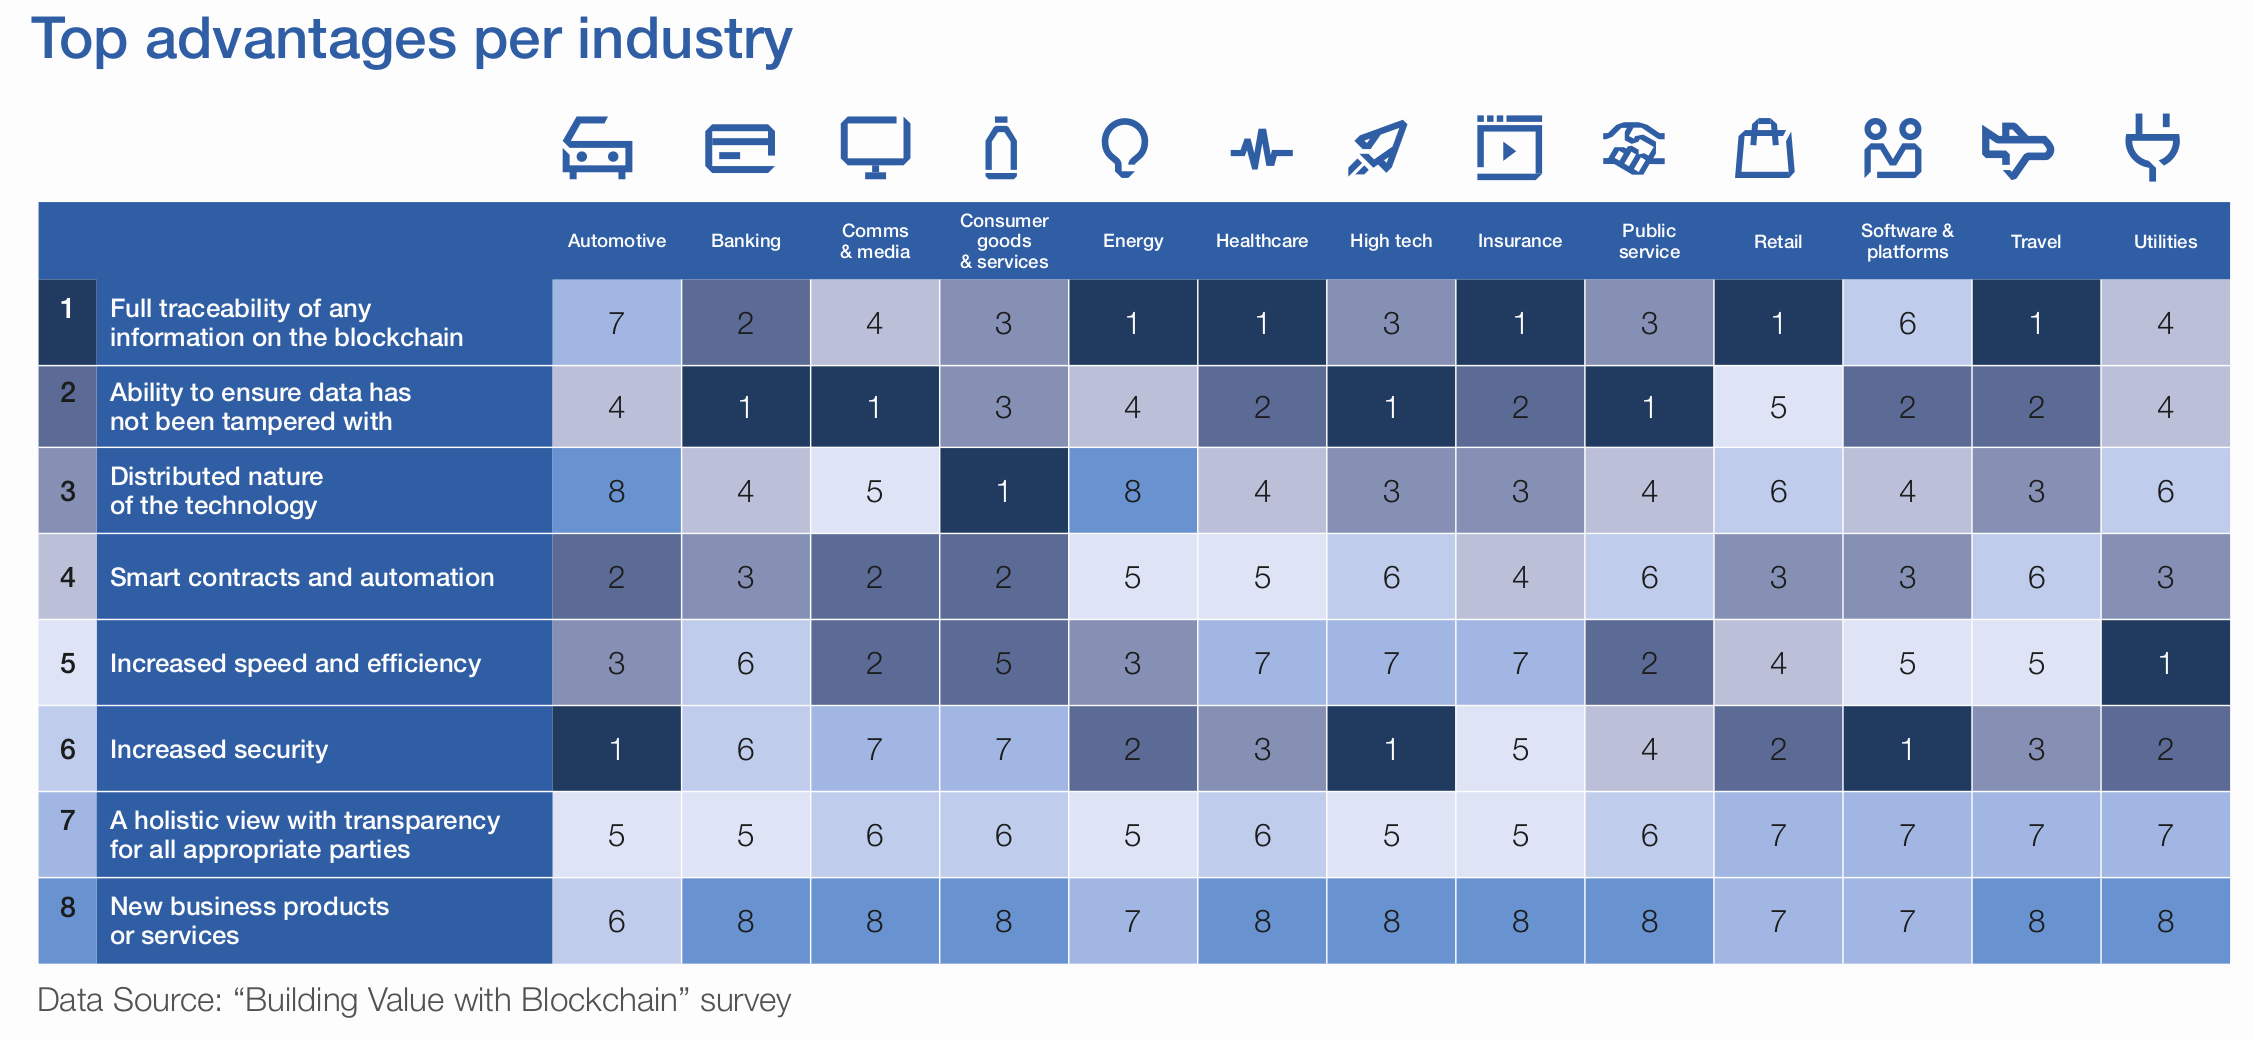
\includegraphics[width=11.5cm]{../pics/blockchain/wef-accenture201906-topadvantage}
    \caption{from the \citeauthor{wef-accenture201906} (\citeyear{wef-accenture201906})}
	\end{figure}
% based on a global survey of 550 individuals across 13 industries, dozens of interviews with public-sector leaders and private-sector chief executive officers, and an analysis of 79 blockchain projects. The projects were evaluated across three main value dimensions: 1) improving productivity and quality; 2) increasing transparency among parties; and 3) reinventing  products and processes.
% (...)
% When asked what led organizations to invest in blockchain technology, 75% included their organizational priority for innovation. The top three areas of interest across surveyed industries were: 1) full traceability of information on the blockchain; 2) the ability to check that data had not been tampered with; and 3) the way the technology is distributed. Notably, few organizations selected “new business products or services” – which ranked last among the options for investment.
}

\frame{
	\frametitle{WEF's Blockchain Value Framework}
	\begin{figure}
		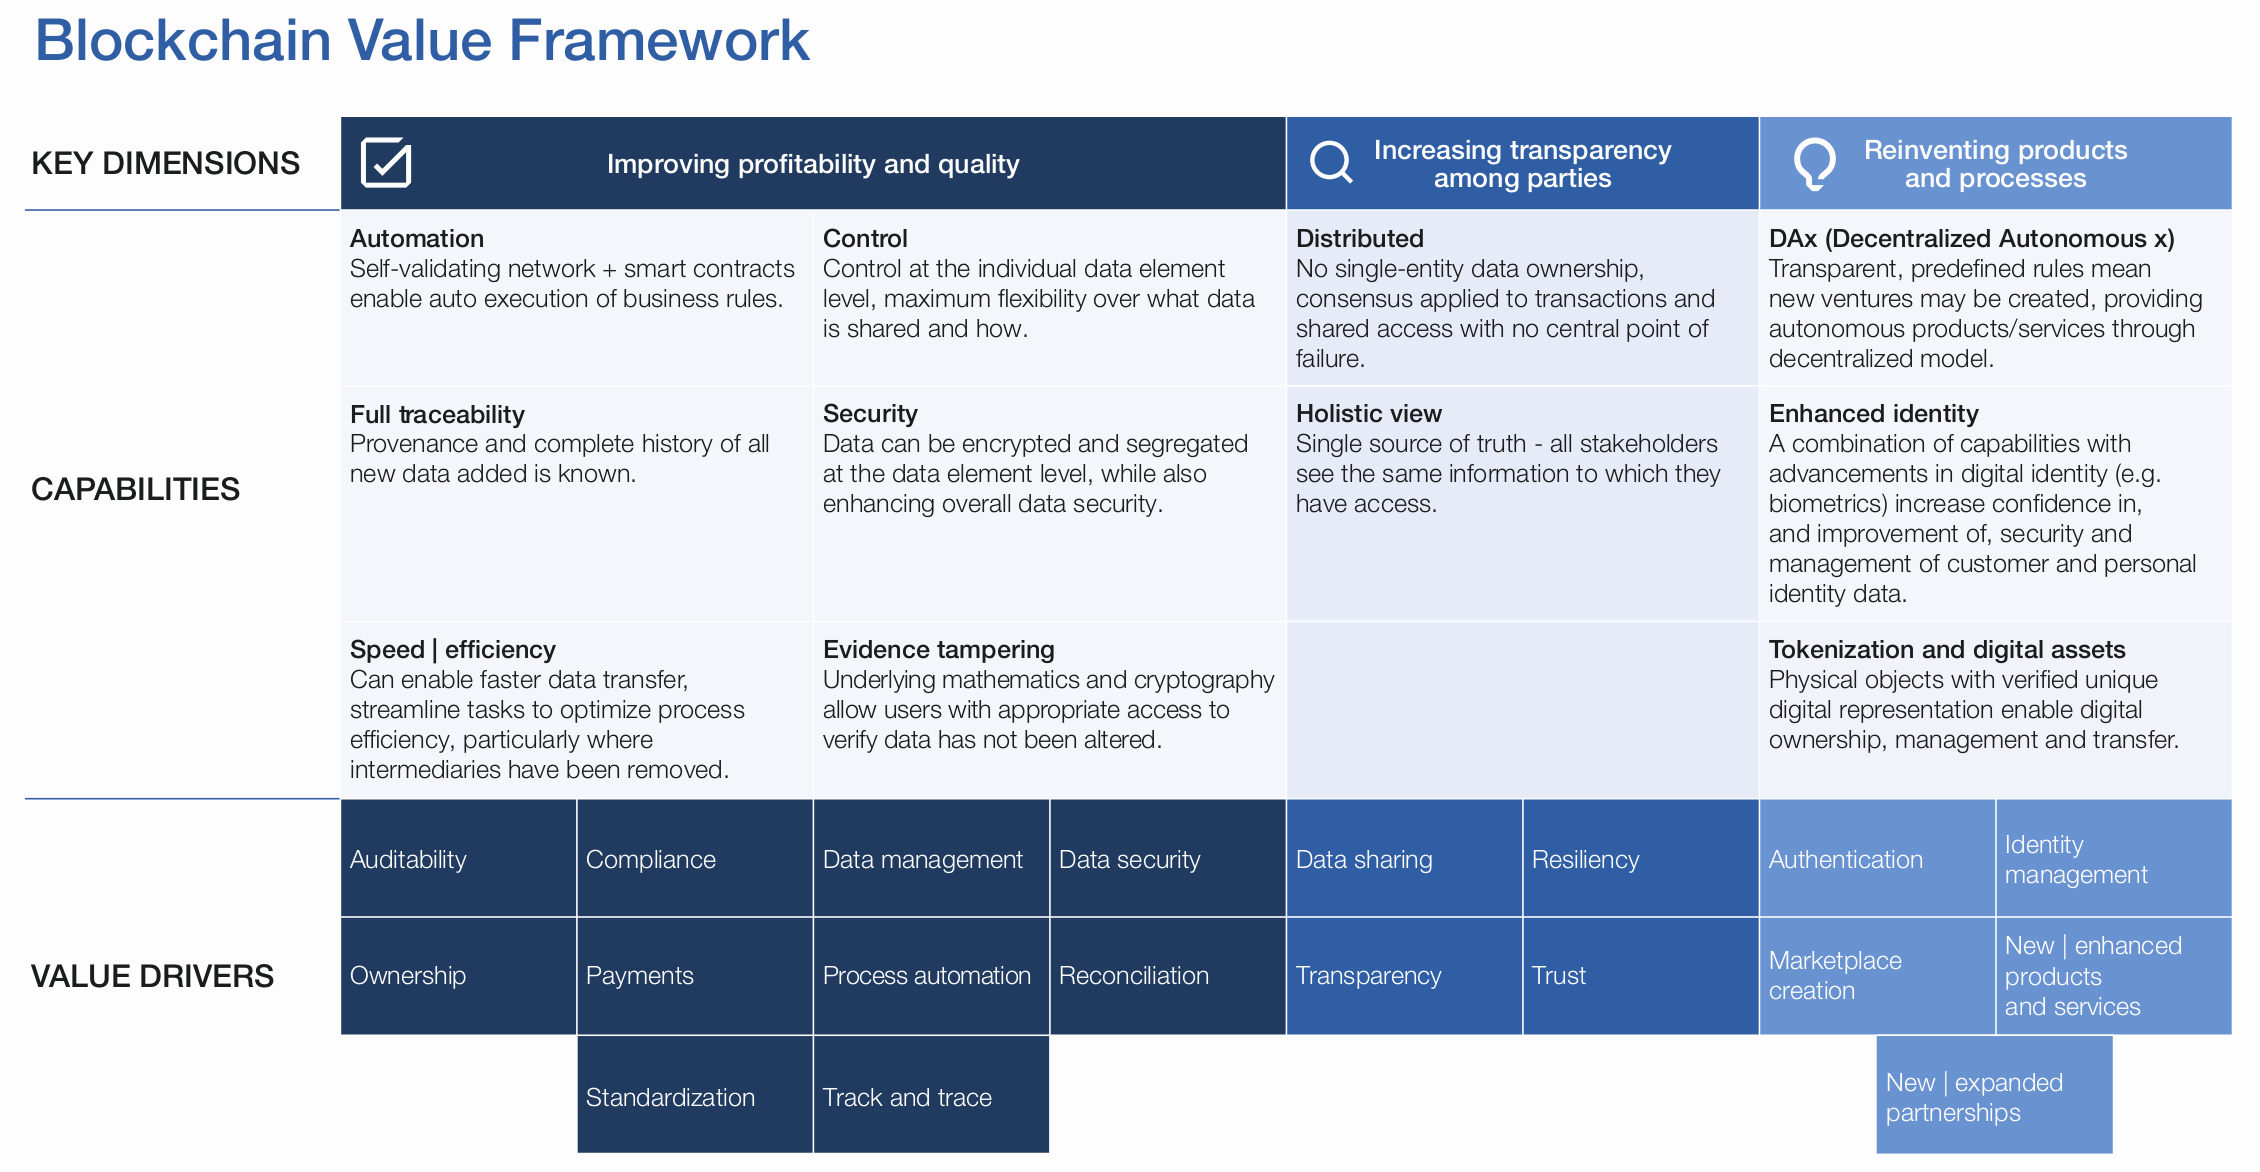
\includegraphics[width=11.5cm]{../pics/blockchain/wef-accenture201906-value-fwk}
    \caption{from the \citeauthor{wef-accenture201906} (\citeyear{wef-accenture201906})}
	\end{figure}
}

% ======================================================================================================
%                         Key institutional usecases
% ======================================================================================================
\section{Key institutional usecases in banking}

%----------------------------------------------------------------------------
\subsection{Banking with or without banks?}
\frame{
	\frametitle{Blockchain: a non-neutral technology enabling a new paradigm}
	\centering\Huge
	Centralized vs Decentralized 
}

\frame{
    \frametitle{Peer-to-peer payments (Bitcoin)}
    \begin{itemize}
        \item Building on years of research \& development (\cite{brunton_digital_2019}),
        \pause
        \item Bitcoin solves the digital payment problem (\cite{nakamoto_bitcoin_2008}),
        \pause
        \item particularly the double-spend problem (\cite{antonopoulos_mastering_2017}), and
        \item every May 25, we celebrate ``Bitcoin Pizza day'', remembering Laszlo Hanyecz who bought two pizzas (worth \$30) for 10,000 BTC on May 25, 2010 (\cite{antonopoulos_mastering_2017}).
    \end{itemize}
}

\frame{
    \frametitle{Bitcoin \& altcoins first usecases}
    \begin{itemize}
    \item \textbf{payment}: this usecase has been slowly adopted but recently reaching mass market with Amazon and Shopify, for example (\cite{jonker_what_2019,matthews_how_2020,schultz_shopify_2020})
    \pause
    \item \textbf{remittances}: it's been very expensive to send money abroad, so much that cutting prices by 5\% would save \$16~bn a year according to the World Bank. The price went down to 6.79\% earlier this year (\cite{noauthor_remittance_2020}). The system (SWIFT) is obsolete, complex, and open to attacks.
    \item \textbf{store of value}: the price of Bitcoin (for example, but crypto-assets are generally correlated) has risen considerably, in spite of its volatility.
    \end{itemize}
}

\frame{
    \frametitle{Blockchain roadmap in banking: the MAS case study (Project Ubin)}
    \begin{figure}
		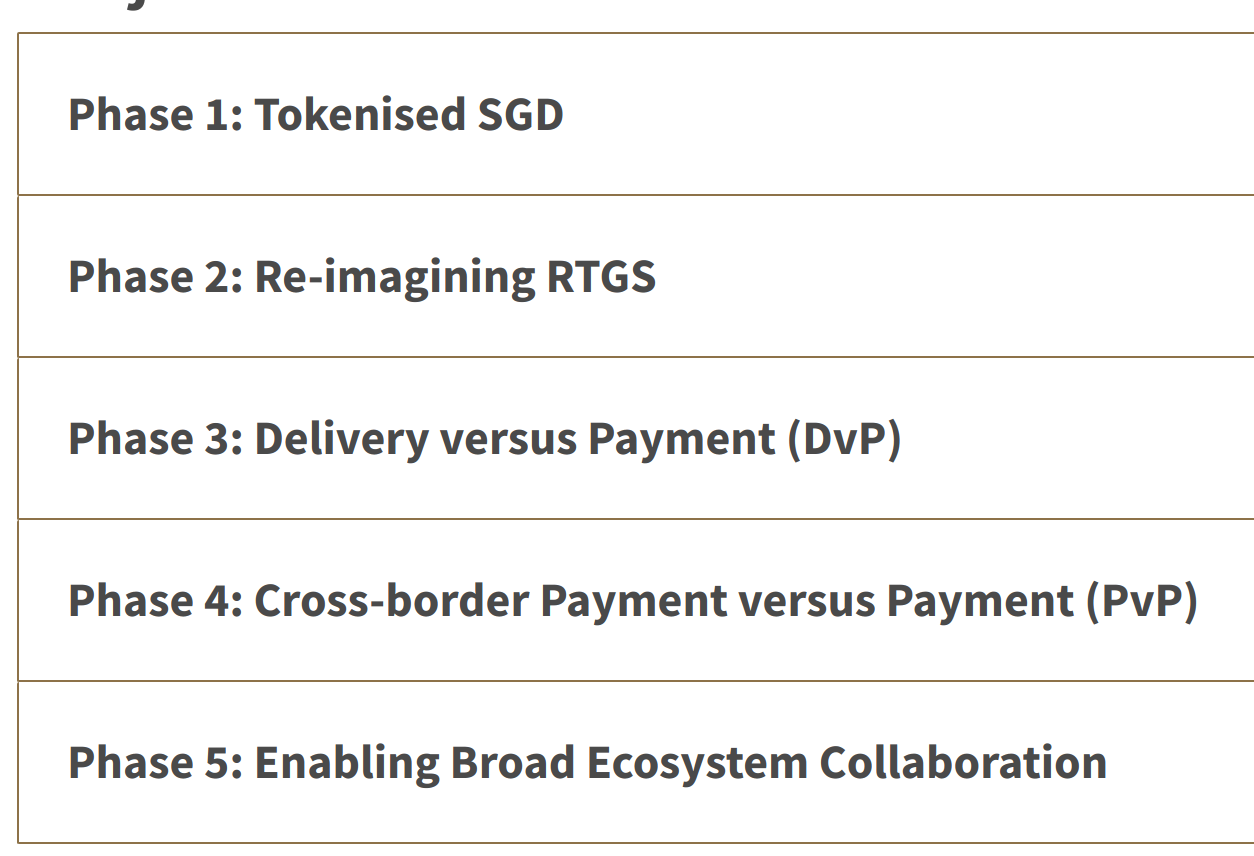
\includegraphics[height=6cm]{../pics/case_studies/mas-ubin/ubin-roadmap}
		\caption{\url{https://www.mas.gov.sg/schemes-and-initiatives/project-ubin}}
	\end{figure}
}

%----------------------------------------------------------------------------
\subsection{Bank-led tokenization of fiat money}
% Phase 1 in the roadmap: 2016-2017 with Deloitte
% From MAS website
% MAS announced on 16 November 2016 that it will be partnering R3, a DLT company, and a consortium of financial institutions on a proof-of-concept project to conduct inter-bank payments using Blockchain technology. The consortium includes the following financial institutions:
% - Bank of America Merrill Lynch
% - Credit Suisse
% - DBS Bank
% - Hongkong and Shanghai Banking Corporation (HSBC) Limited
% - JP Morgan
% - Mitsubishi UFJ Financial Group
% - OCBC 
% - R3
% - Singapore Exchange (SGX)
% - United Overseas Bank (UOB)
\frame{
    \frametitle{Tokenizing fiat money}
    \begin{block}{MAS phase 1 and similar}
        \begin{itemize}
        \item Project Ubin (2016--2017) with Deloitte at the Monetary Authority of Singapore
        \item Project i2i (2018) with ConsenSys, Union Bank, and 80 rural banks in the Philipines (phase 1: bank-to-client and client-to-client, phase 2: commercial bank transactions, phase 3: central bank-issued crypto-peso)
        \item QCAD (2020), and CAD-coin (considered in 2017)
        \end{itemize}
    \end{block}
}





%----------------------------------------------------------------------------
\subsection{Real-Time Gross Settlement}
% Phase 2 in the roadmap: 2017-2018
% MAS and The Association of Banks in Singapore (ABS) announced on 5 October 2017 that the consortium which they are leading had successfully developed software prototype of three different models for decentralised inter-bank payment and settlements with liquidity savings mechanisms. 
% Financial Institutions
% - Bank of America Merrill Lynch
% - Citi
% - Credit Suisse
% - DBS Bank Ltd
% - HSBC Ltd
% - JP Morgan
% - Mitsubishi UFJ Financial Group
% - OCBC Bank
% - SGX
% - Standard Chartered Bank
% - UOB
% 
% Technology Partners
% Technology partners	Scope of appointment
% Accenture	            Manage and develop prototypes
% R3                    Support on the Corda DLT platform
% IBM	                Support on the Hyperledger Fabric DLT platform
% ConsenSys	            Support on the Quorum DLT platform
% Microsoft	            Deployment of prototypes on Azure Blockchain
\frame{
    \frametitle{Real-Time Gross Settlement (RTGS)}
    \begin{block}{MAS phase 2}
        In 2018, MAS runs experiments on several platforms with Accenture and other tech partners: 
        \begin{itemize}
        \item R3 (Corda)
        \item IBM (Hyperledger Fabric)
        \item ConsenSys (Quorum)
        \item Microsoft (Azure Blockchain).
        \end{itemize}
    \end{block}
    \vspace{1em}
    Clients include: Bank of America Merrill Lynch, Citi, Credit Suisse, DBS Bank Ltd, HSBC Ltd, and JP Morgan.
}

\frame{
    \frametitle{Real-Time Gross Settlement (RTGS)}
    The same year (2018), ConsenSys' client SARB is awarded for its RTGS system on a modified version of Quorum.
  	\begin{figure}
		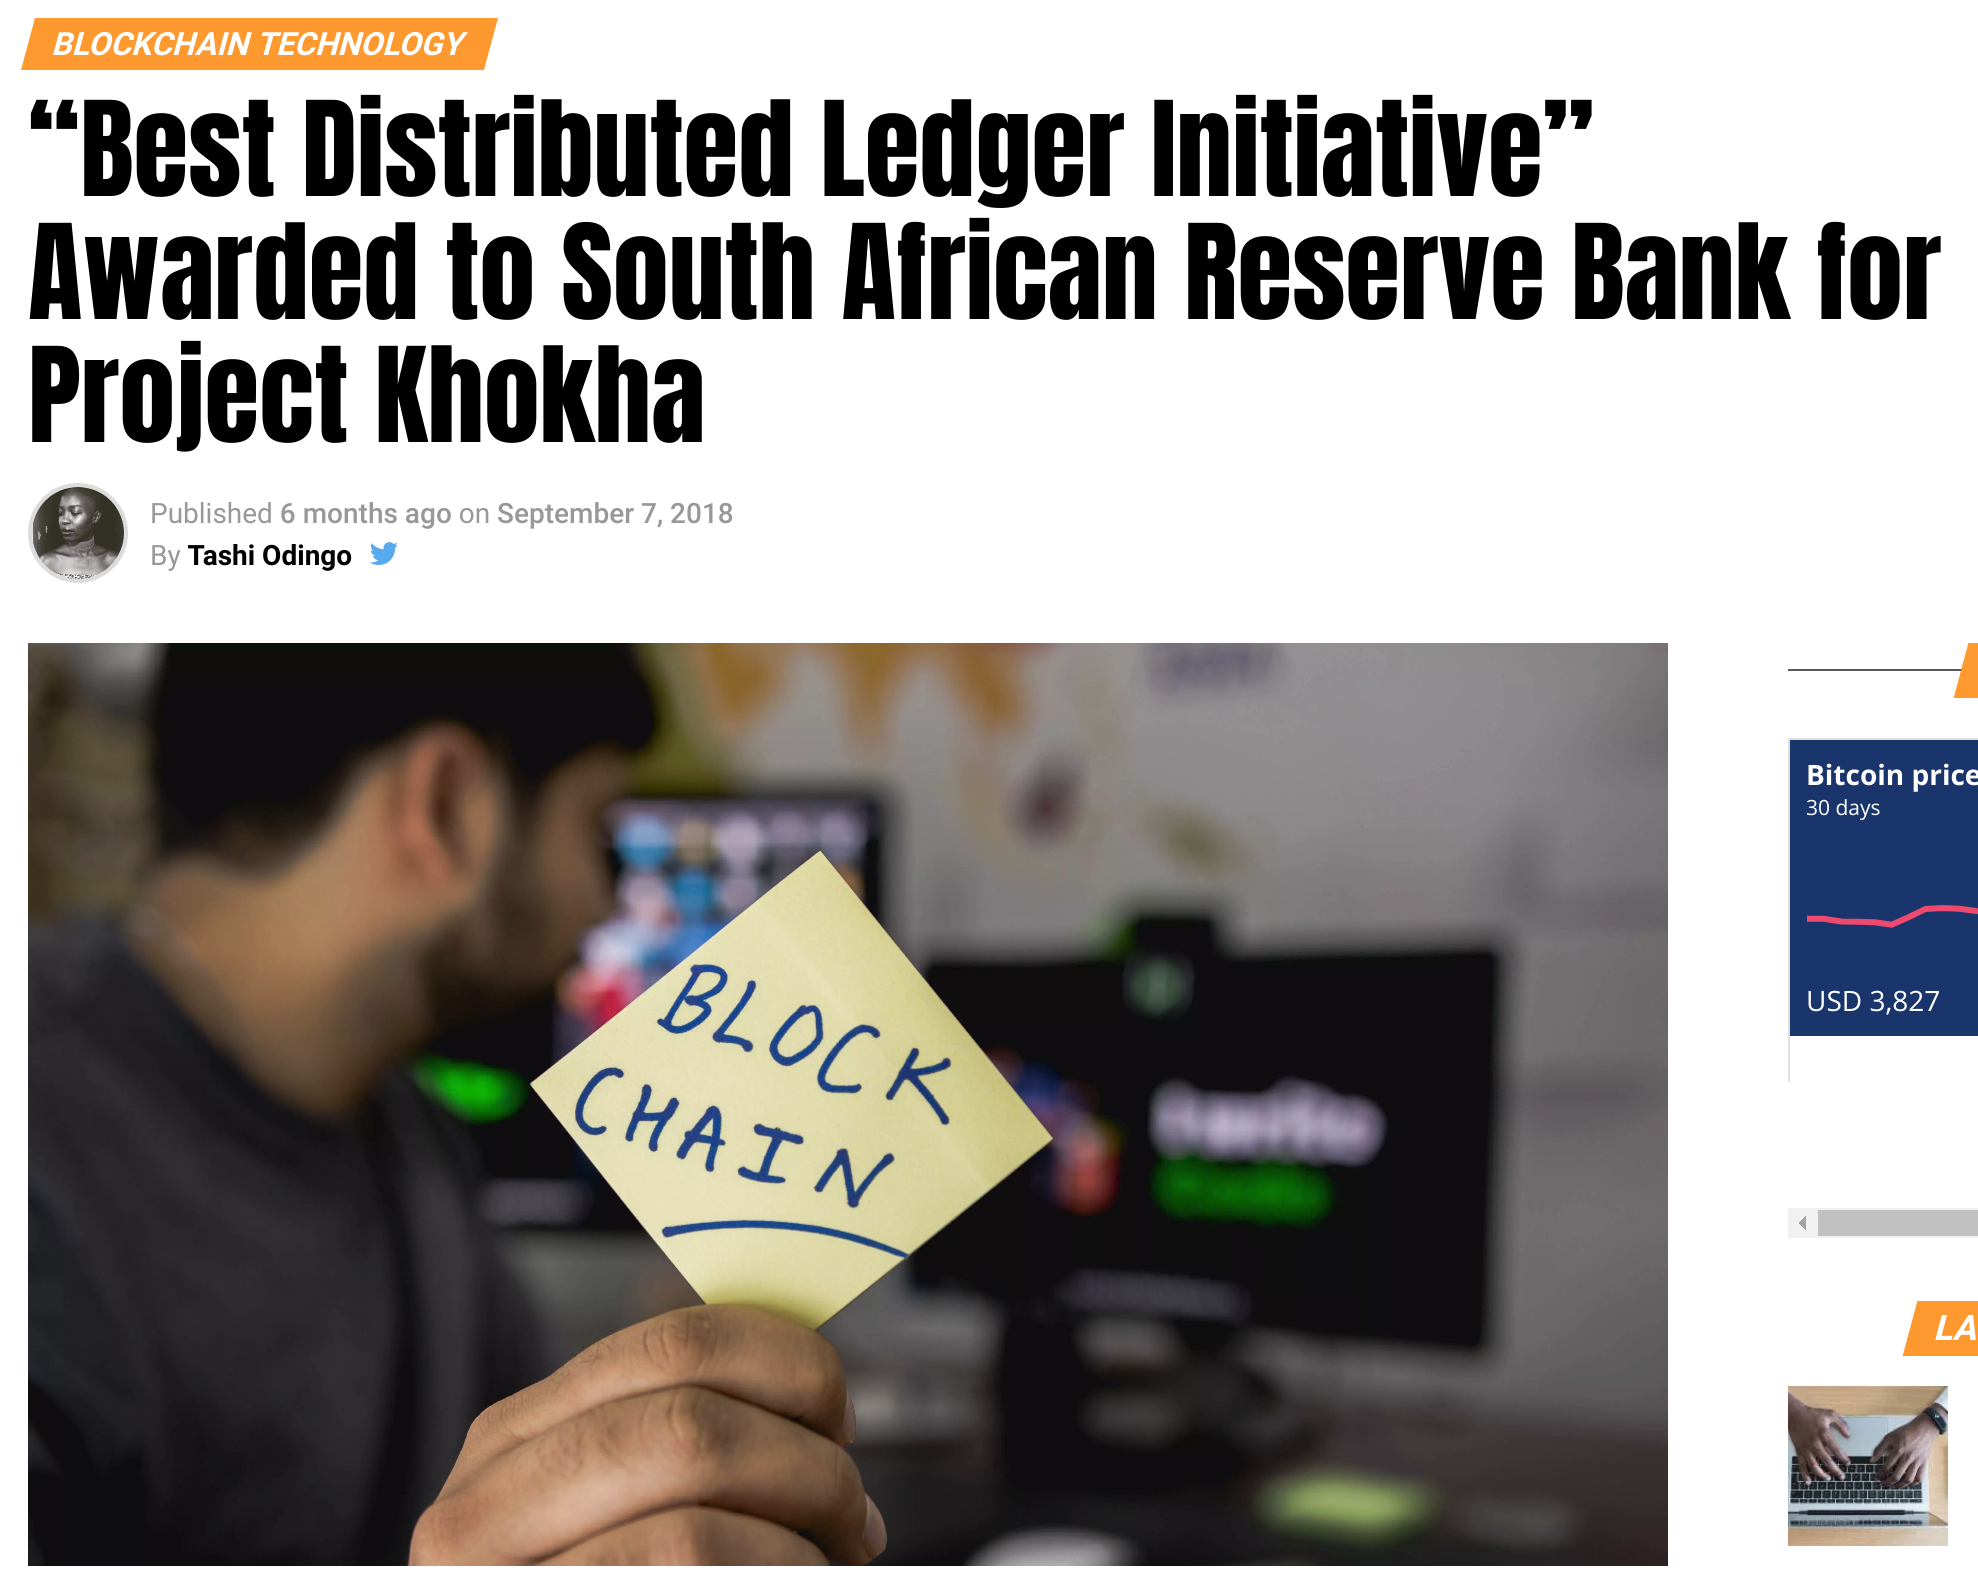
\includegraphics[height=6cm]{../pics/ConsenSys/case_studies/khokha-best-regtech}
		\caption{See the 80-page long report (\cite{noauthor_project_2018})}
	\end{figure}
}

%----------------------------------------------------------------------------
\subsection{Delivery vs Payment (DvP)}
% Phase 3 in 2018
% MAS and Singapore Exchange (SGX) announced on 24 August 2018 that it is collaborating to develop Delivery versus Payment (DvP) capabilities for settlement of tokenised assets across different blockchain platforms.
% This will allow financial institutions and corporate investors to carry out simultaneous exchange and final settlement of tokenised digital currencies and securities assets, improving operational efficiency and reducing settlement risks. Three companies, Anquan, Deloitte and Nasdaq were appointed as technology partners for this project. They will leverage the open-source software developed and made publicly available in Project Ubin Phase 2.
\frame{
    \frametitle{Delivery vs Payment (DvP)}
    In 2018, the MAS built upon their open source code from the previous phase to complete a DvP project with Anquan, Deloitte and Nasdaq.
  	\begin{figure}
		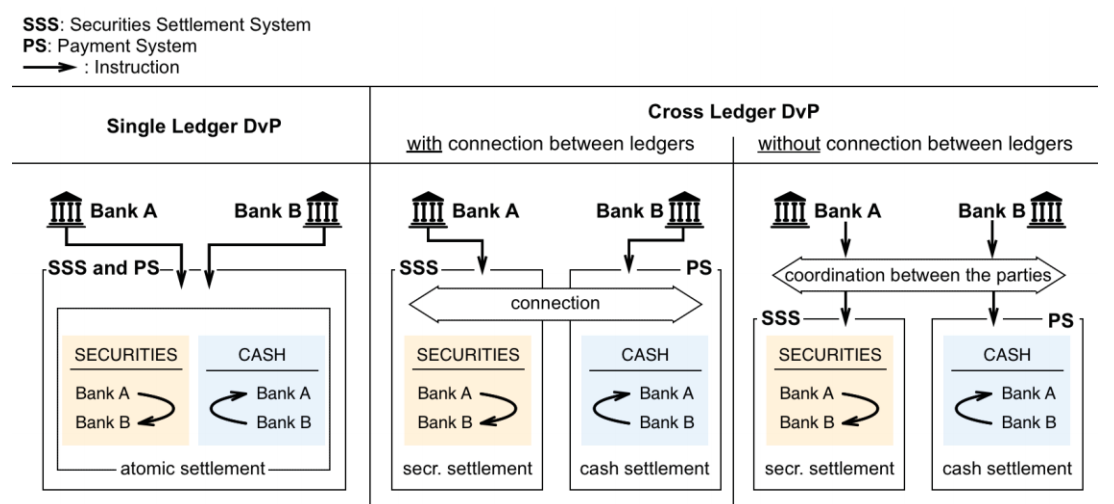
\includegraphics[width=11cm]{../pics/big_banks/ecb-japan-dvp-approaches}
		\caption{extract from \href{https://www.ecb.europa.eu/pub/pdf/other/stella_project_report_march_2018.pdf}{a report on Stella, a project with the ECB and the Bank of Japan}}
	\end{figure}
}

%----------------------------------------------------------------------------
\subsection{Cross-border payment vs Payment (PvP)}
% Phase 4: 2018 and 2019
% The Bank of Canada (BoC), Bank of England (BoE) and the MAS jointly published a report on 15 November 2018 which assesses alternative models that could enhance cross-border payments and settlements. The report examines existing challenges and considers alternative models that could in time result in improvements in speed, cost and transparency for users.
% The report, Cross-border interbank payments and settlements: Emerging opportunities for digital transformation  (4.4 MB), provides an initial framework for the global financial community to assess cross-border payments and settlements in greater depth. Specifically, it discusses how a variety of payment models could be implemented, from both a technical and non-technical perspective.
% MAS and BoC subsequently linked up their respective experimental domestic payment networks, namely Project Jasper and Project Ubin, and announced on 2 May 2019 a successful experiment on cross-border and cross-currency payments using central bank digital currencies. MAS and BoC jointly published a report, Jasper-Ubin Design Paper: Enabling Cross-Border High Value Transfer using DLT  (2.45 MB), which proposes different design options for cross-border settlement systems.
\frame{
    \frametitle{Cross-border payment vs Payment (PvP)}
    \begin{block}{MAS phase 4}
        \begin{itemize}
        \item 2018: Bank of Canada (BoC), Bank of England (BoE) and the MAS explore cross-border payments and settlements
        \item 2019: MAS and BoC link Project Ubin and Project Jasper using central bank digital currencies
        \end{itemize}    
    \end{block}
}

\frame{
    \frametitle{Cross-border payment history \& market size}
    \begin{itemize}
    \item Ripple has worked in this niche for a decade (\cite{armknecht_ripple_2015,burniske_cryptoassets_2017})
    \item R3 Consortium dates to 2014
    \item In 2018, HSBC moved \$250~bn in assets through crypto rails, using Stellar, linking 50 banks in 72 countries (\cite{mearian_ibm_2019})
    \item Cross-border transactions amounted to \$23.7 trillion worldwide in 2018 (\cite{li_how_2019})
    \item A top usecase for banks today (\cite{noauthor_new_2019})
    \end{itemize}
}

%----------------------------------------------------------------------------
\subsection{Multiple currencies}
\frame{
    \frametitle{Broadening the ecosystem}
    \begin{block}{MAS phase 5}
        Completed in 2019, with J.P. Morgan and Temasek, the prototype handles multiple currencies on the same network.
        Features include
        \begin{itemize}
        \item Delivery-versus-Payment (DvP) settlement with private exchanges
        \item conditional payments and escrow for trade
        \item payment commitments for trade finance.
        \end{itemize}
    \end{block}
}

%----------------------------------------------------------------------------
\subsection{Trade Finance}
\frame{
    \frametitle{Trade Finance}
  	\begin{figure}
		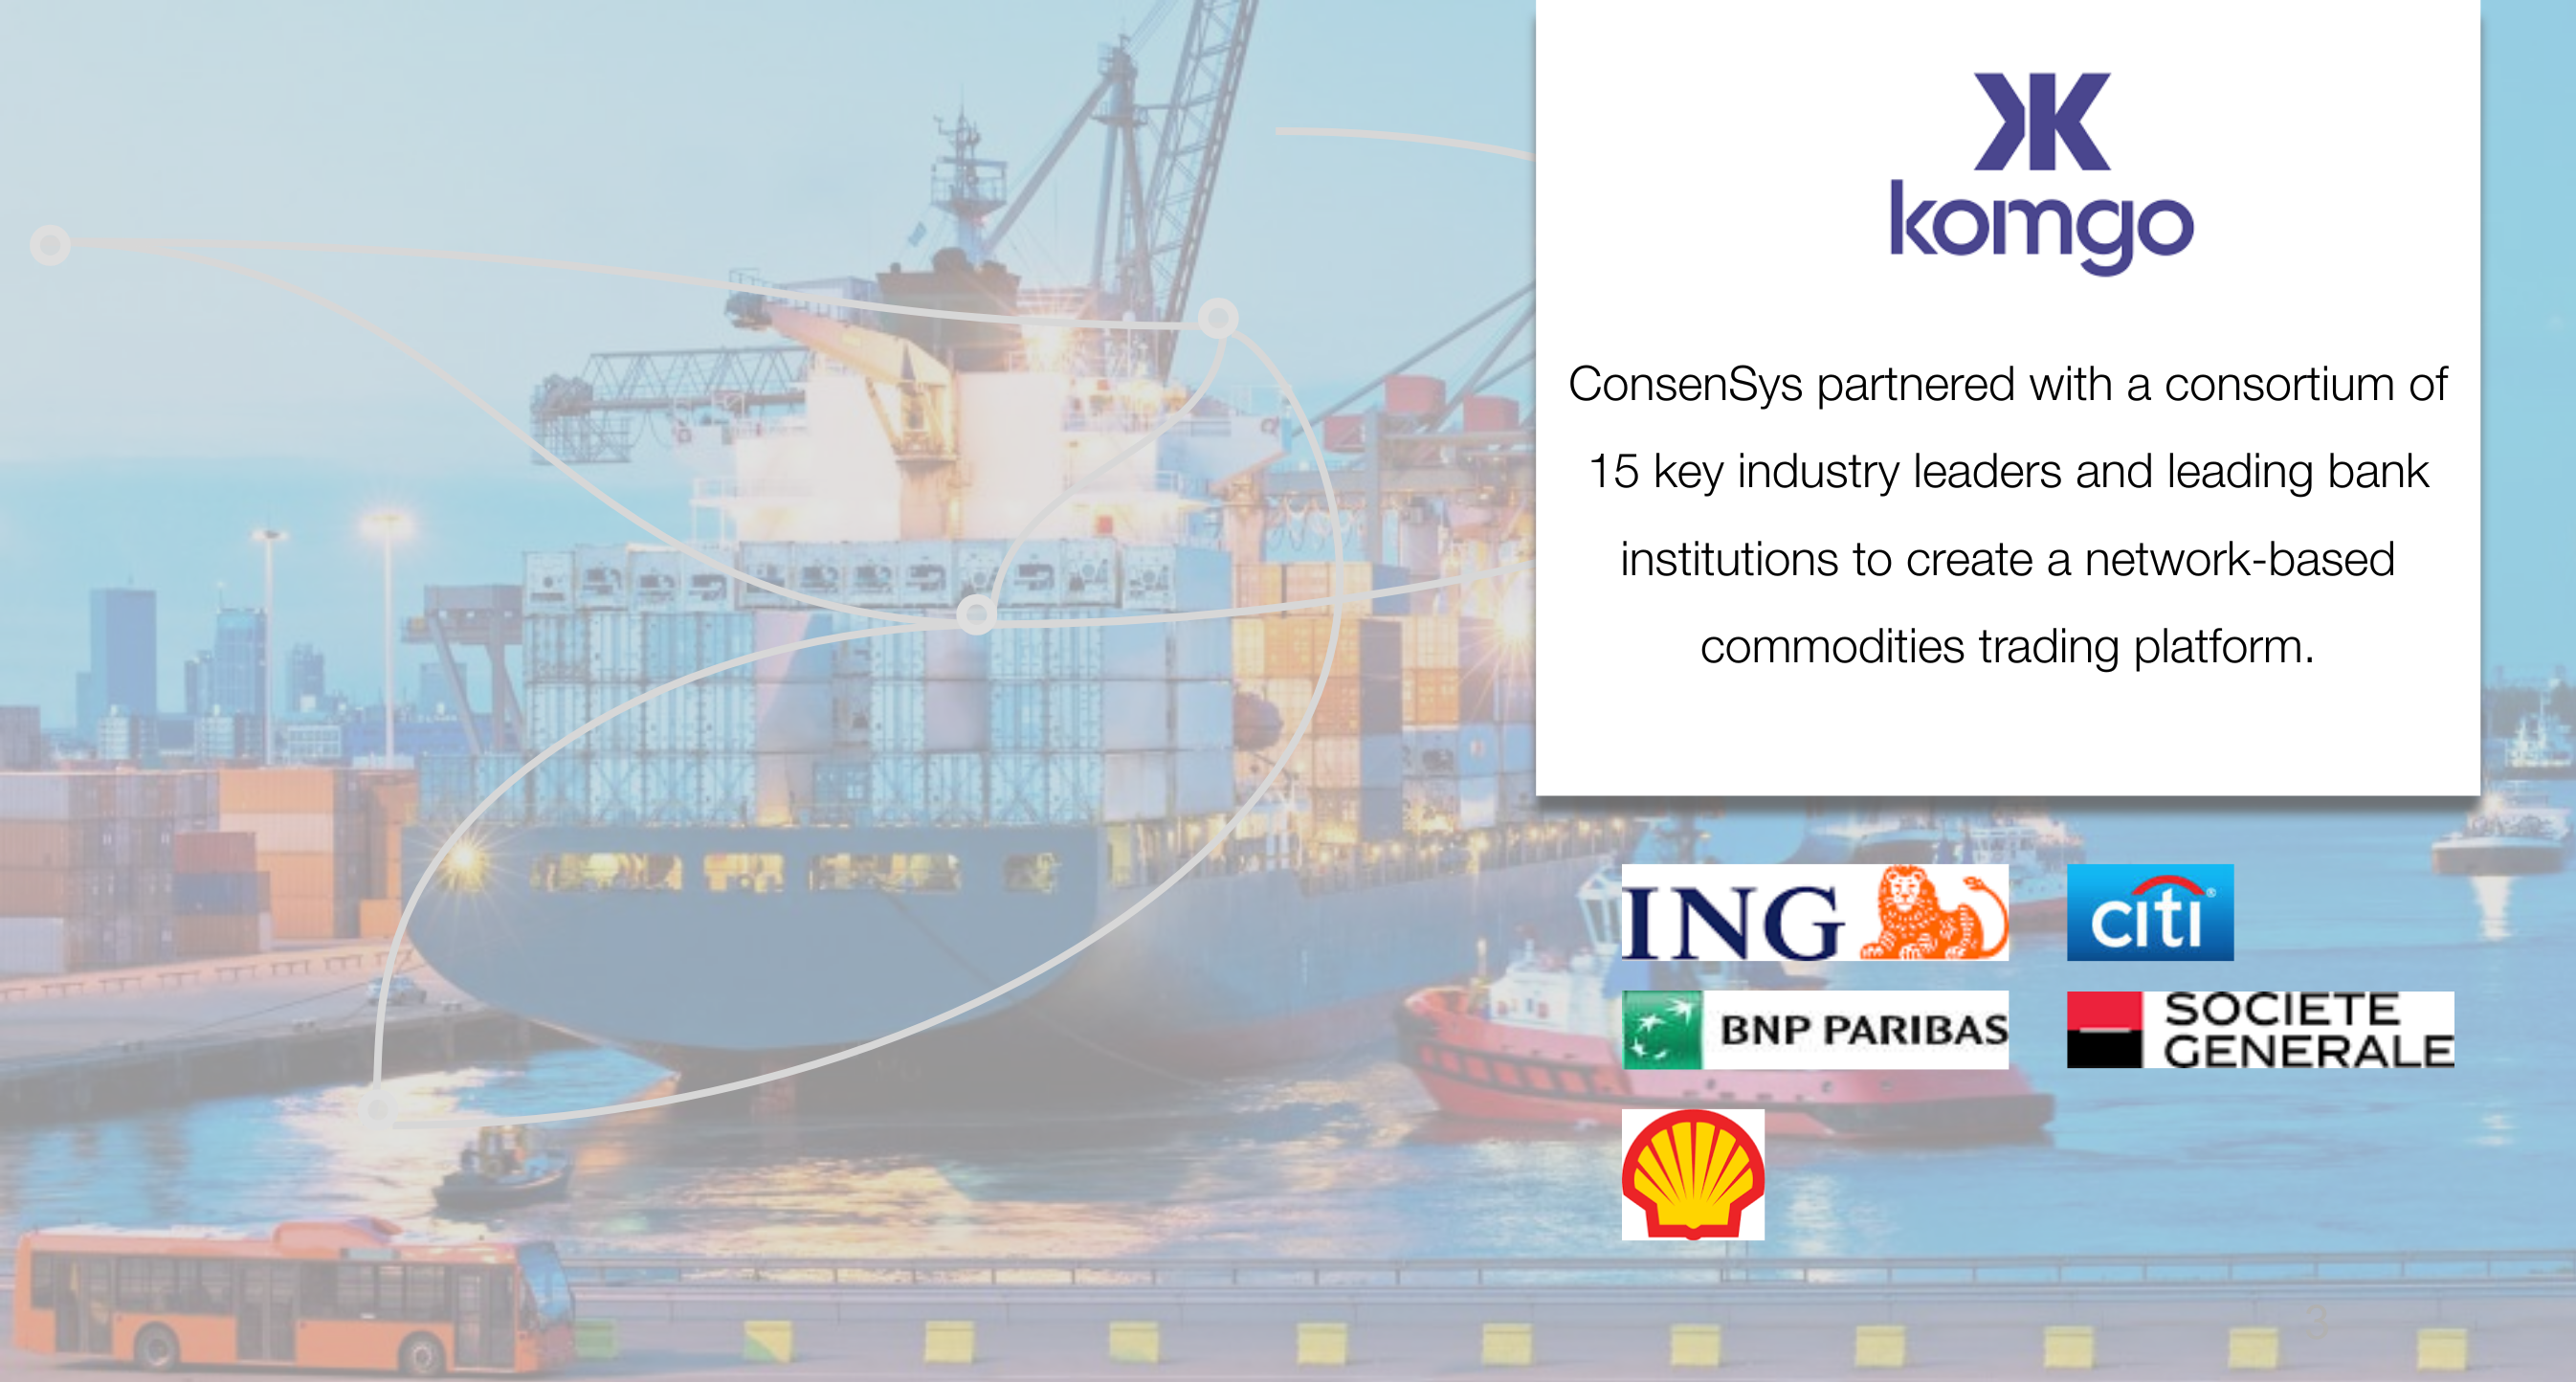
\includegraphics[height=6cm]{../pics/ConsenSys/case_studies/komgo}
	\end{figure}
}

\frame{
	\frametitle{Case Study: Ontario farmers sell corn on Blockchain rails}
	\framesubtitle{\tiny\url{https://farmtario.com/crops/ontario-farmers-make-first-blockchain-system-corn-sale/}}
	\begin{figure}
	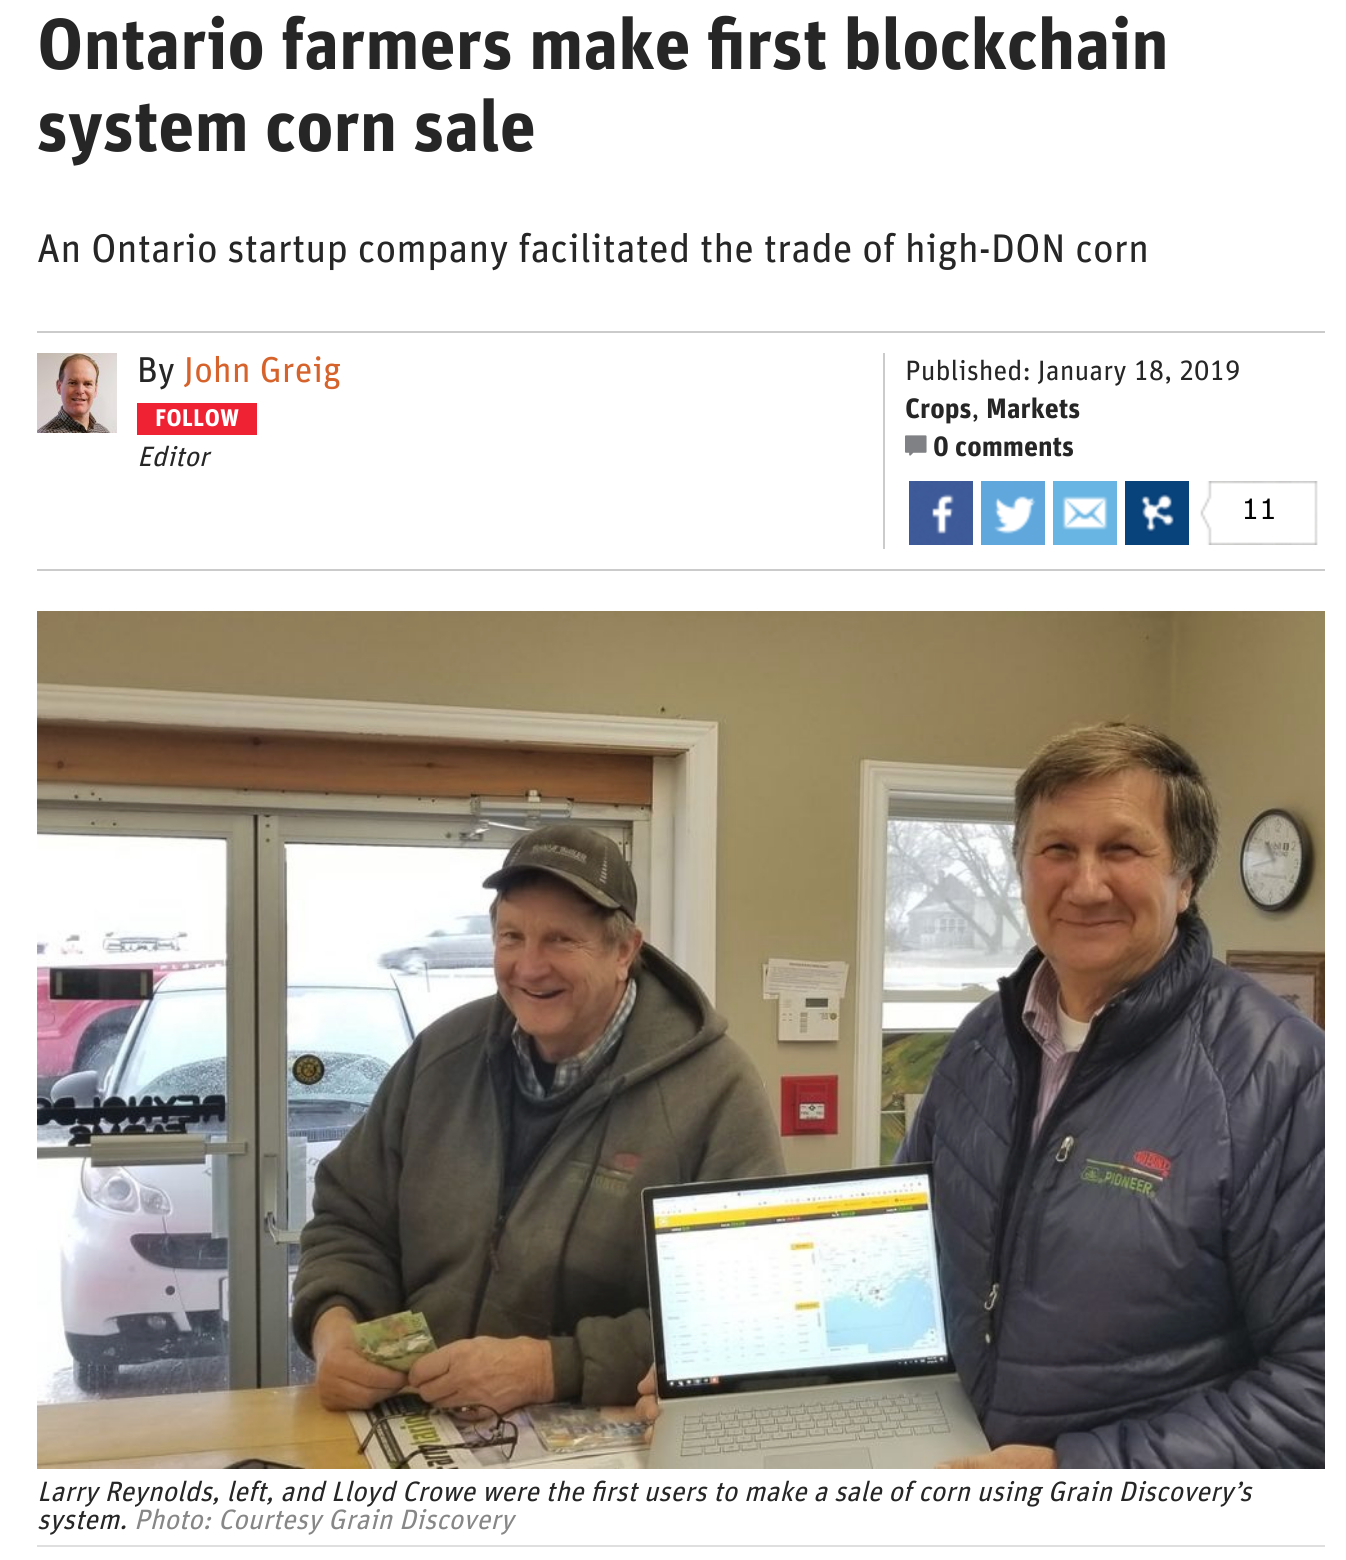
\includegraphics[height=6cm]{../pics/case_studies/ontario-farmers-corn2019}
	\end{figure}
}

%----------------------------------------------------------------------------
\subsection{Capital markets}
\frame{
    \frametitle{Investment in Crypto-Assets}
    \begin{itemize}
    \item Fidelity opens the market in Europe where legislation allows (\cite{wilson_fidelity_2020})
    \item 3iQ provides funds with exposure to Bitcoin and Ether in Canada (\url{https://3iq.ca})
    \item RBC is exploring
    \end{itemize}
}

%----------------------------------------------------------------------------
\subsection{Identity Management}

\frame{
	\frametitle{Identity Management: logging to Service Canada}
	\begin{figure}
		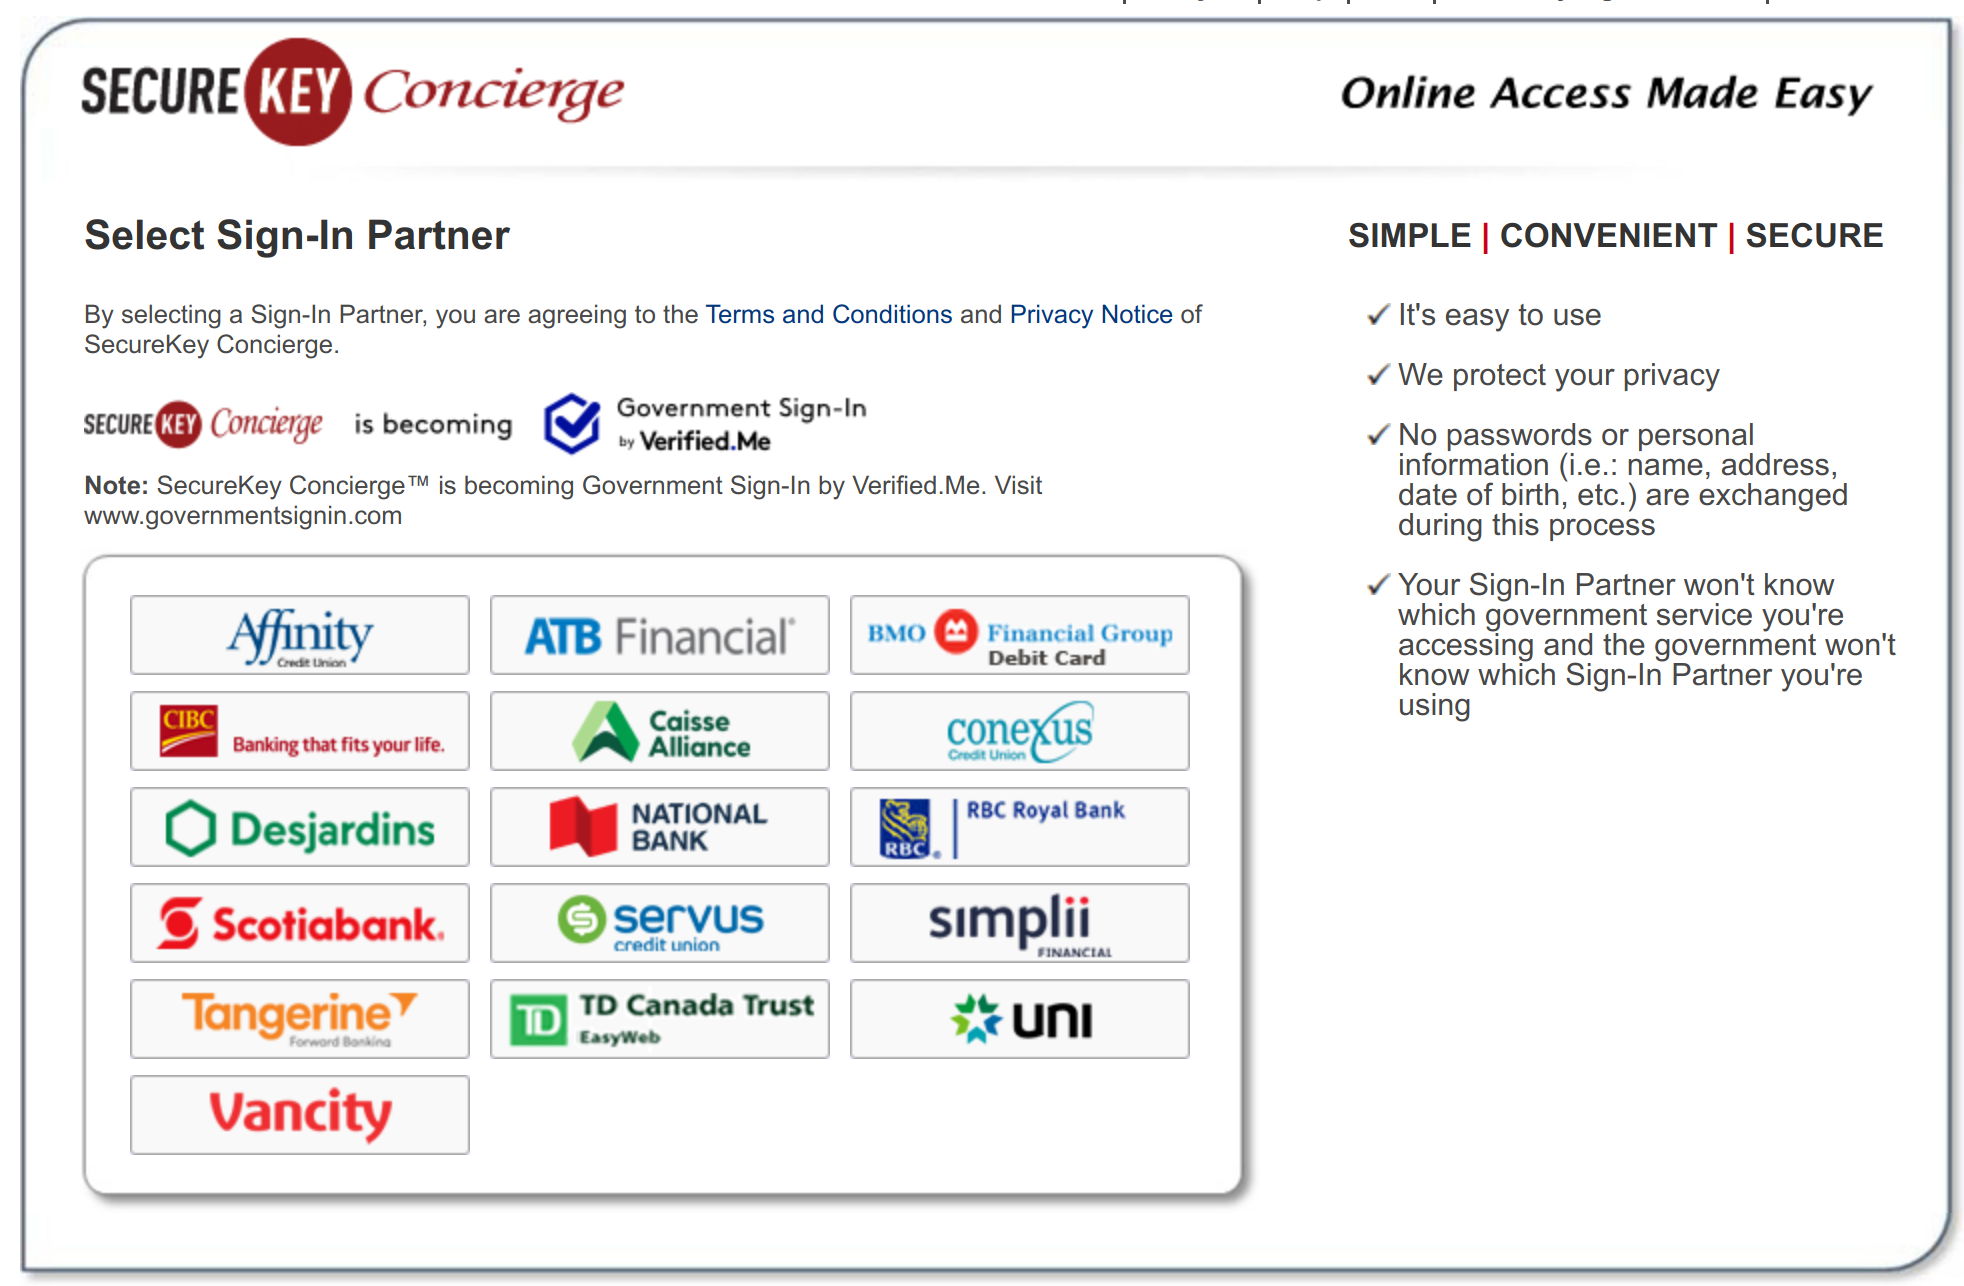
\includegraphics[height=6cm]{../pics/identity/securekey-login-to-servicecanada}
	\end{figure}
}

\frame{
	\frametitle{Self-Sovereign Identity}
	\framesubtitle{Extract from the white paper from \cite{sovrin-white-paper}}
	\begin{figure}
		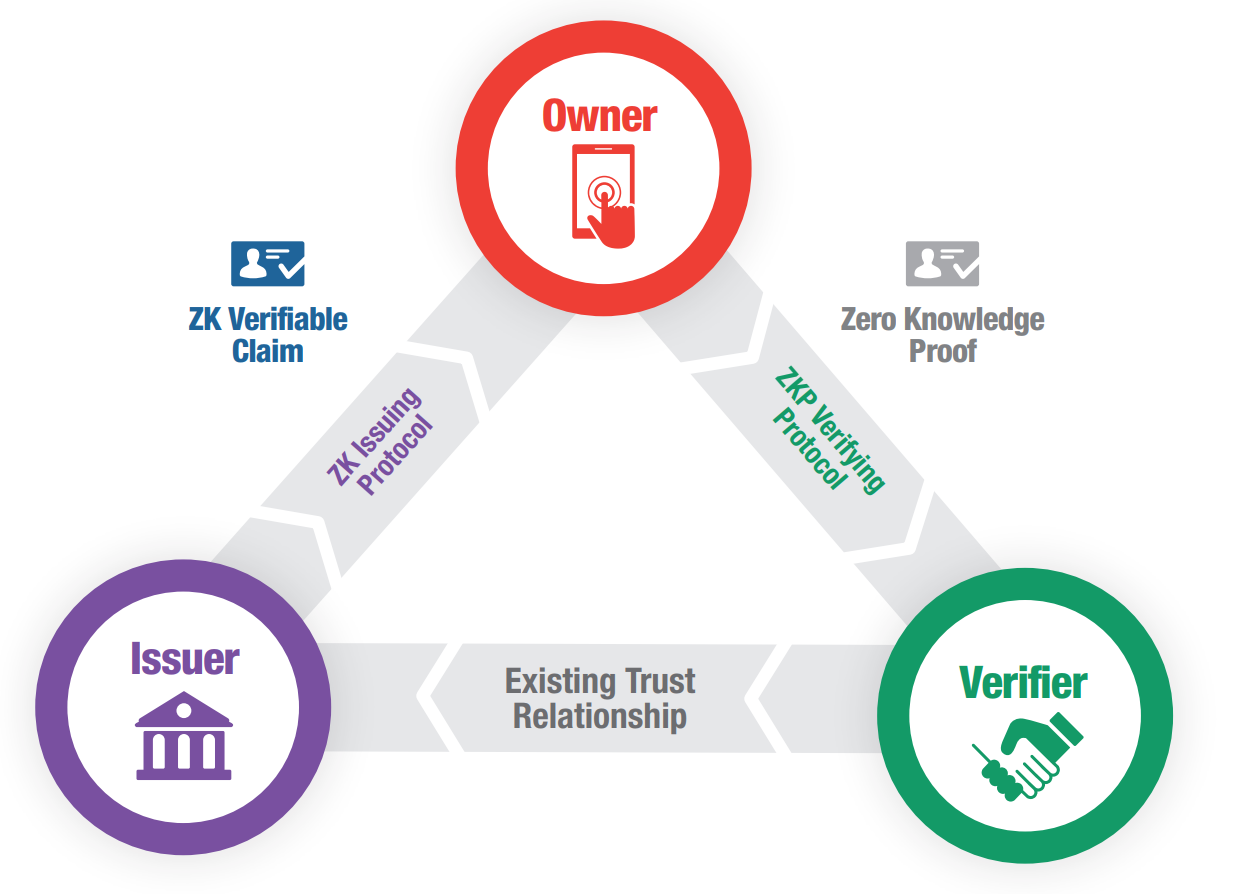
\includegraphics[height=6cm]{../pics/identity/sovrin-zkp}
	\end{figure}
}

\frame{
	\frametitle{The first e-bike service worldwide powered by decentralized identity}
	\framesubtitle{See full article from \cite{nawfal2019:uport-bike}}
	% https://medium.com/uport/zug-residents-can-now-ride-e-bikes-using-their-uport-powered-zug-digital-ids-7ed31ac9d621
	% see also Zug eID launch -- https://www.ethnews.com/zug-and-uport-see-first-citizens-identity-registered-on-the-ethereum-blockchain
	\begin{figure}
		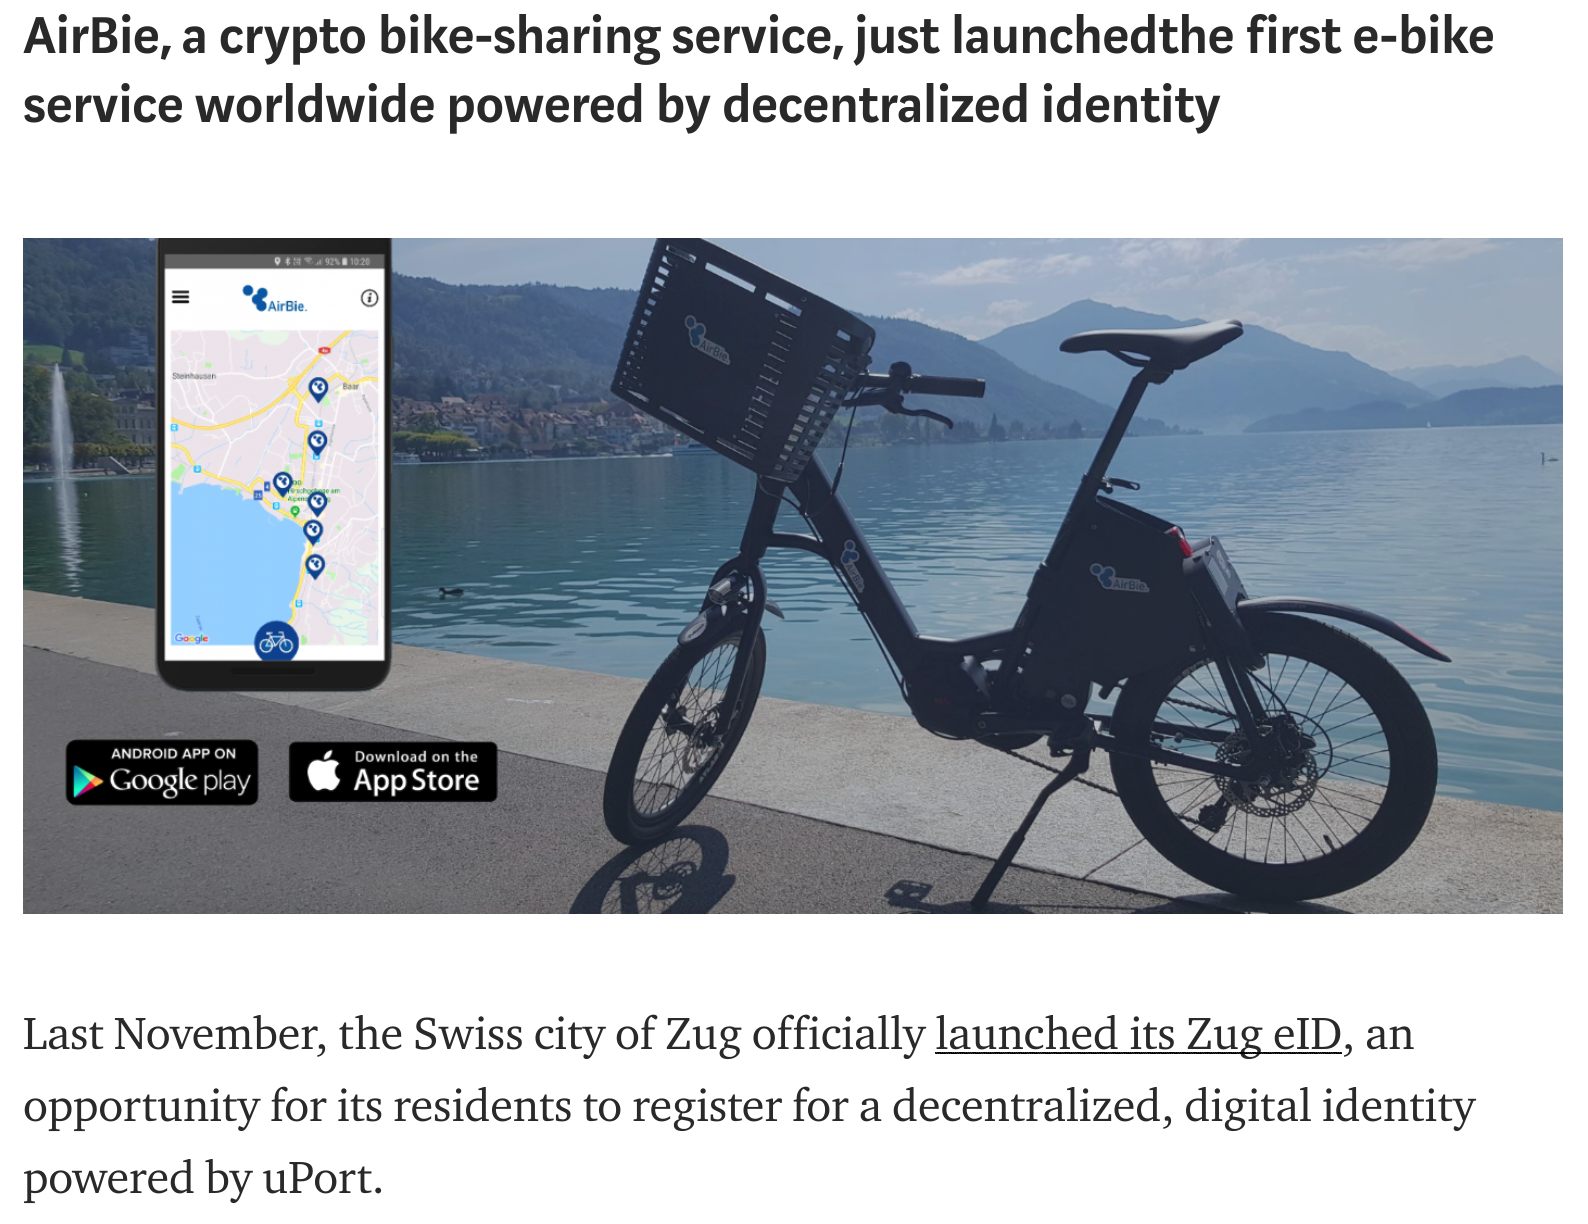
\includegraphics[height=6cm]{../pics/identity/uport-bike}
	\end{figure}
}

\frame{
	\frametitle{SSI in Alberta}
	\begin{figure}
		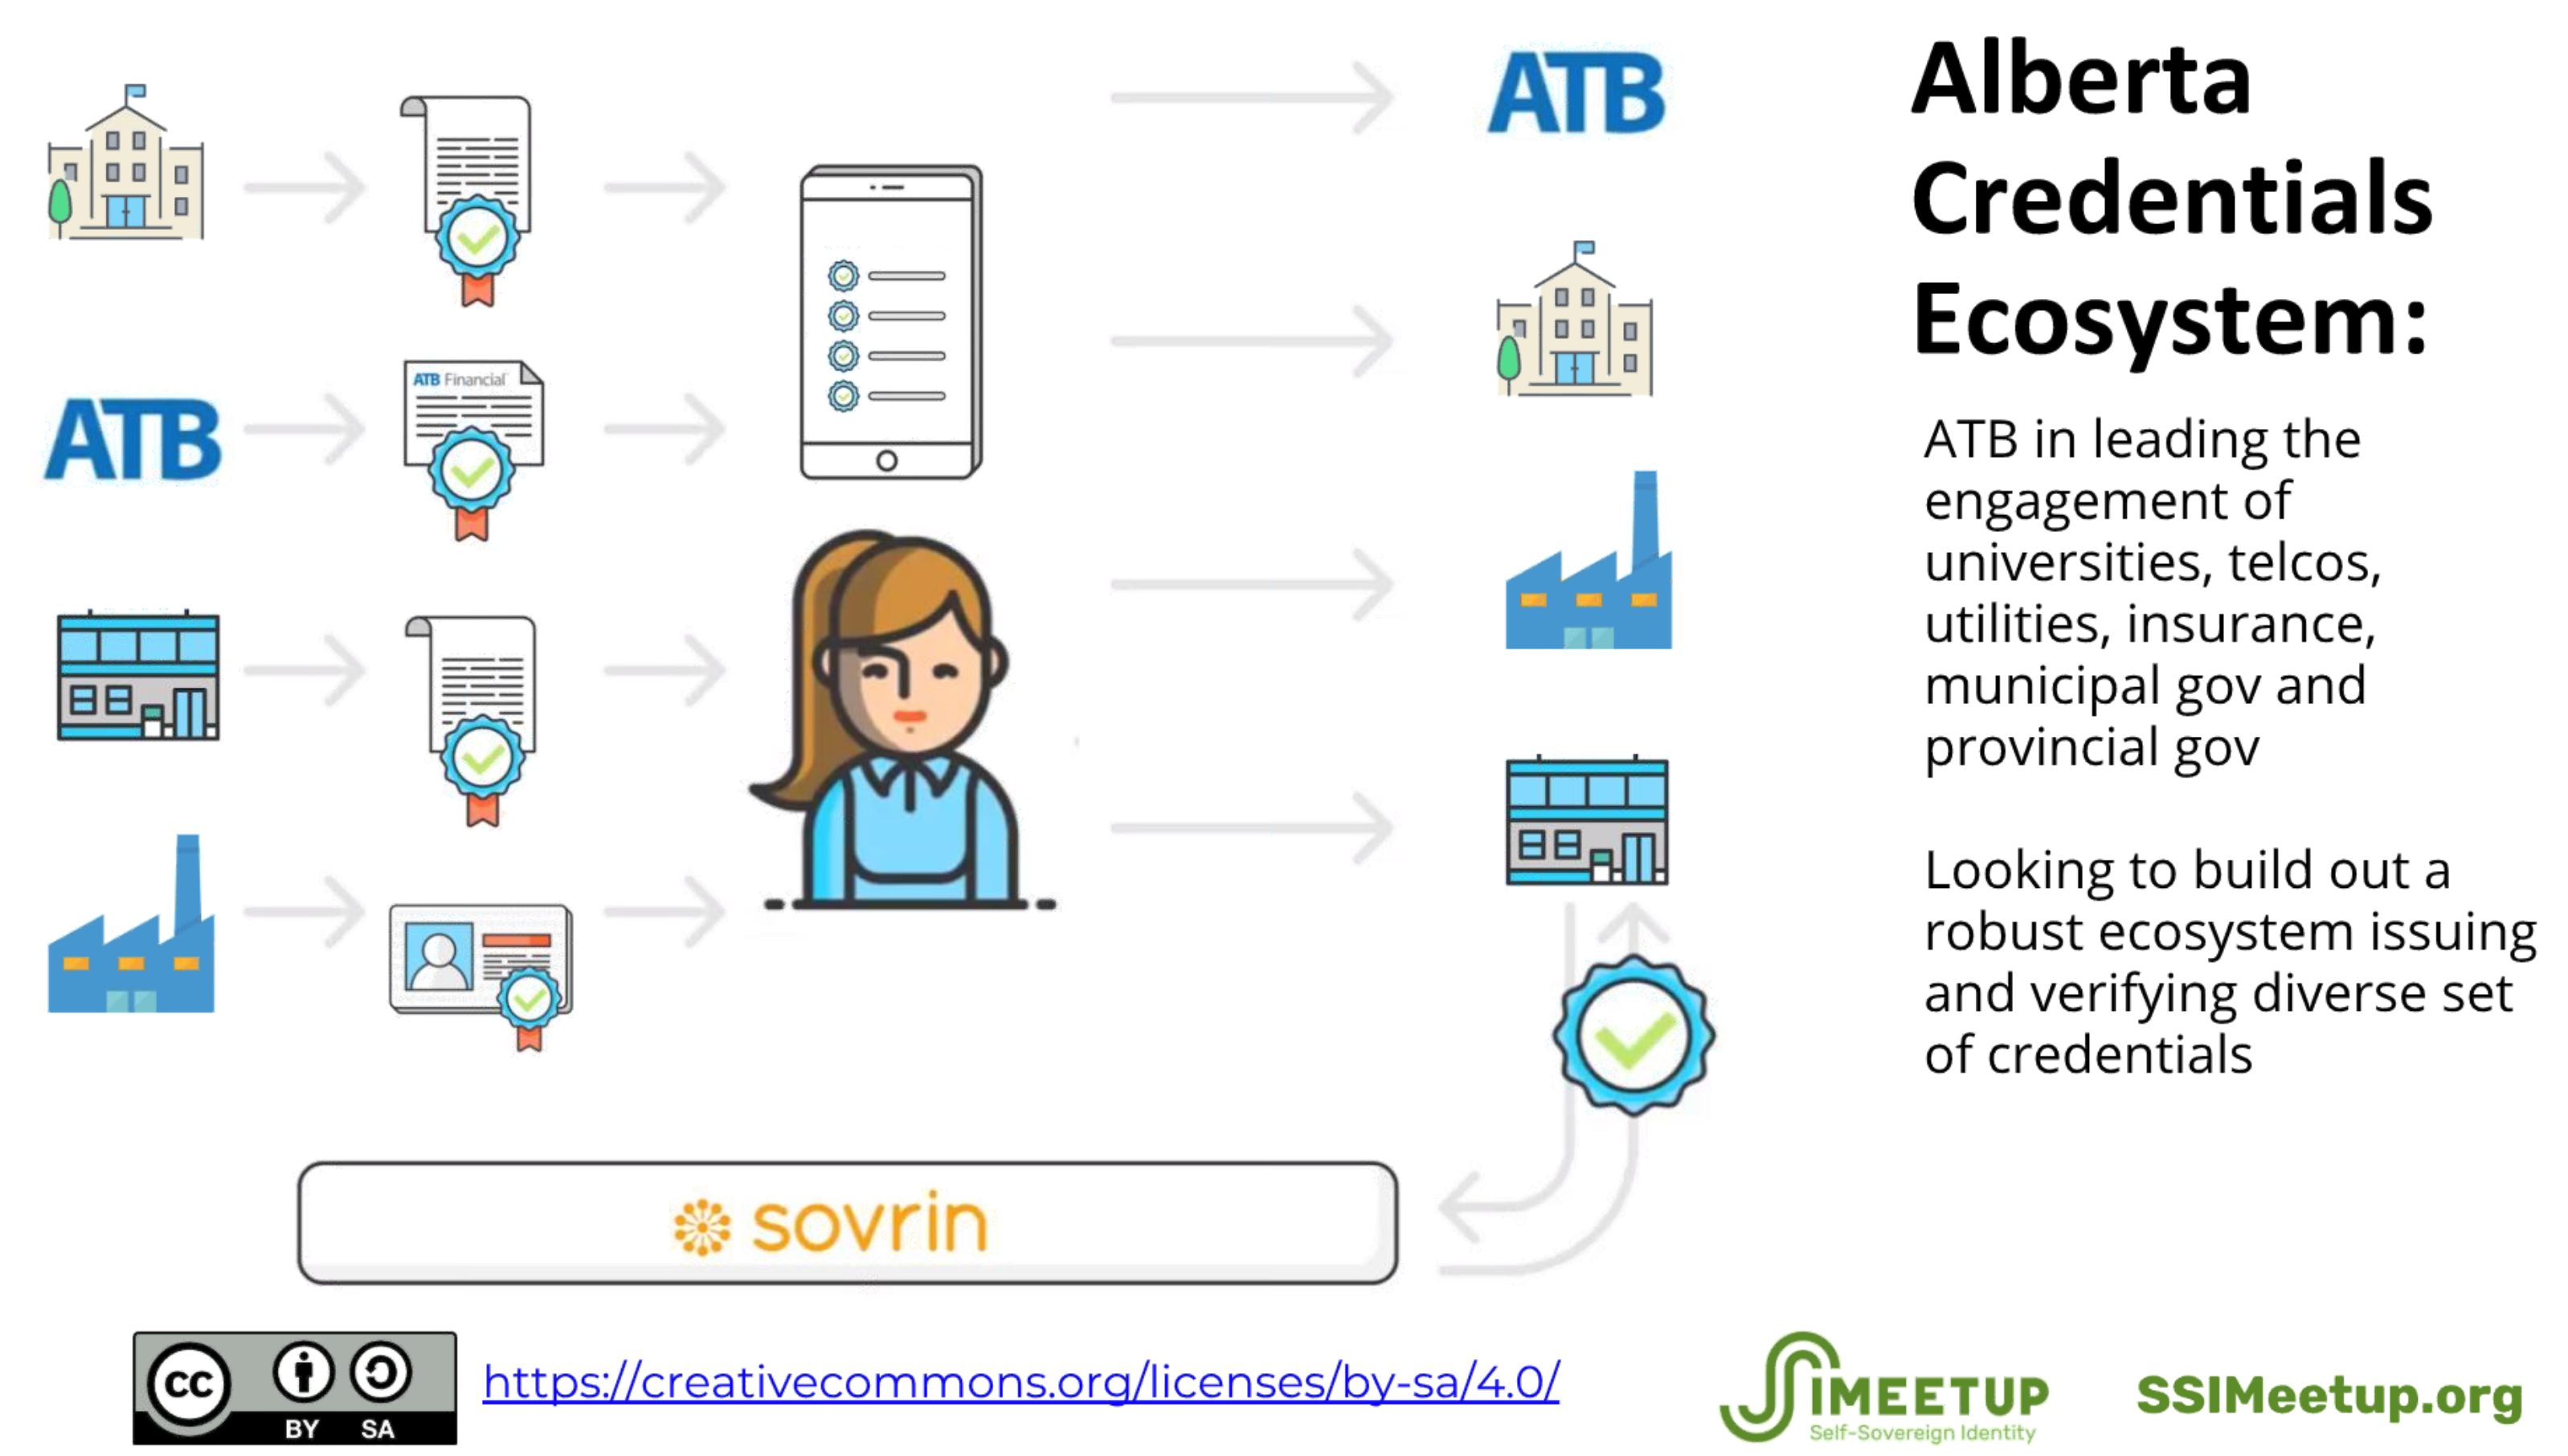
\includegraphics[height=6cm]{../pics/case_studies/alberta-credentials-ecosystem}
		\captionsetup{justification=centering}
		\caption{from \cite{ssimeetup201902:atb-slides}}
	\end{figure}
}

% ======================================================================================================
%                         Global Money 
% ======================================================================================================
\section{World money} 
\subsection{A global stable coin?}
\frame{
  \frametitle{Libra}
	\begin{figure}
        \centering
		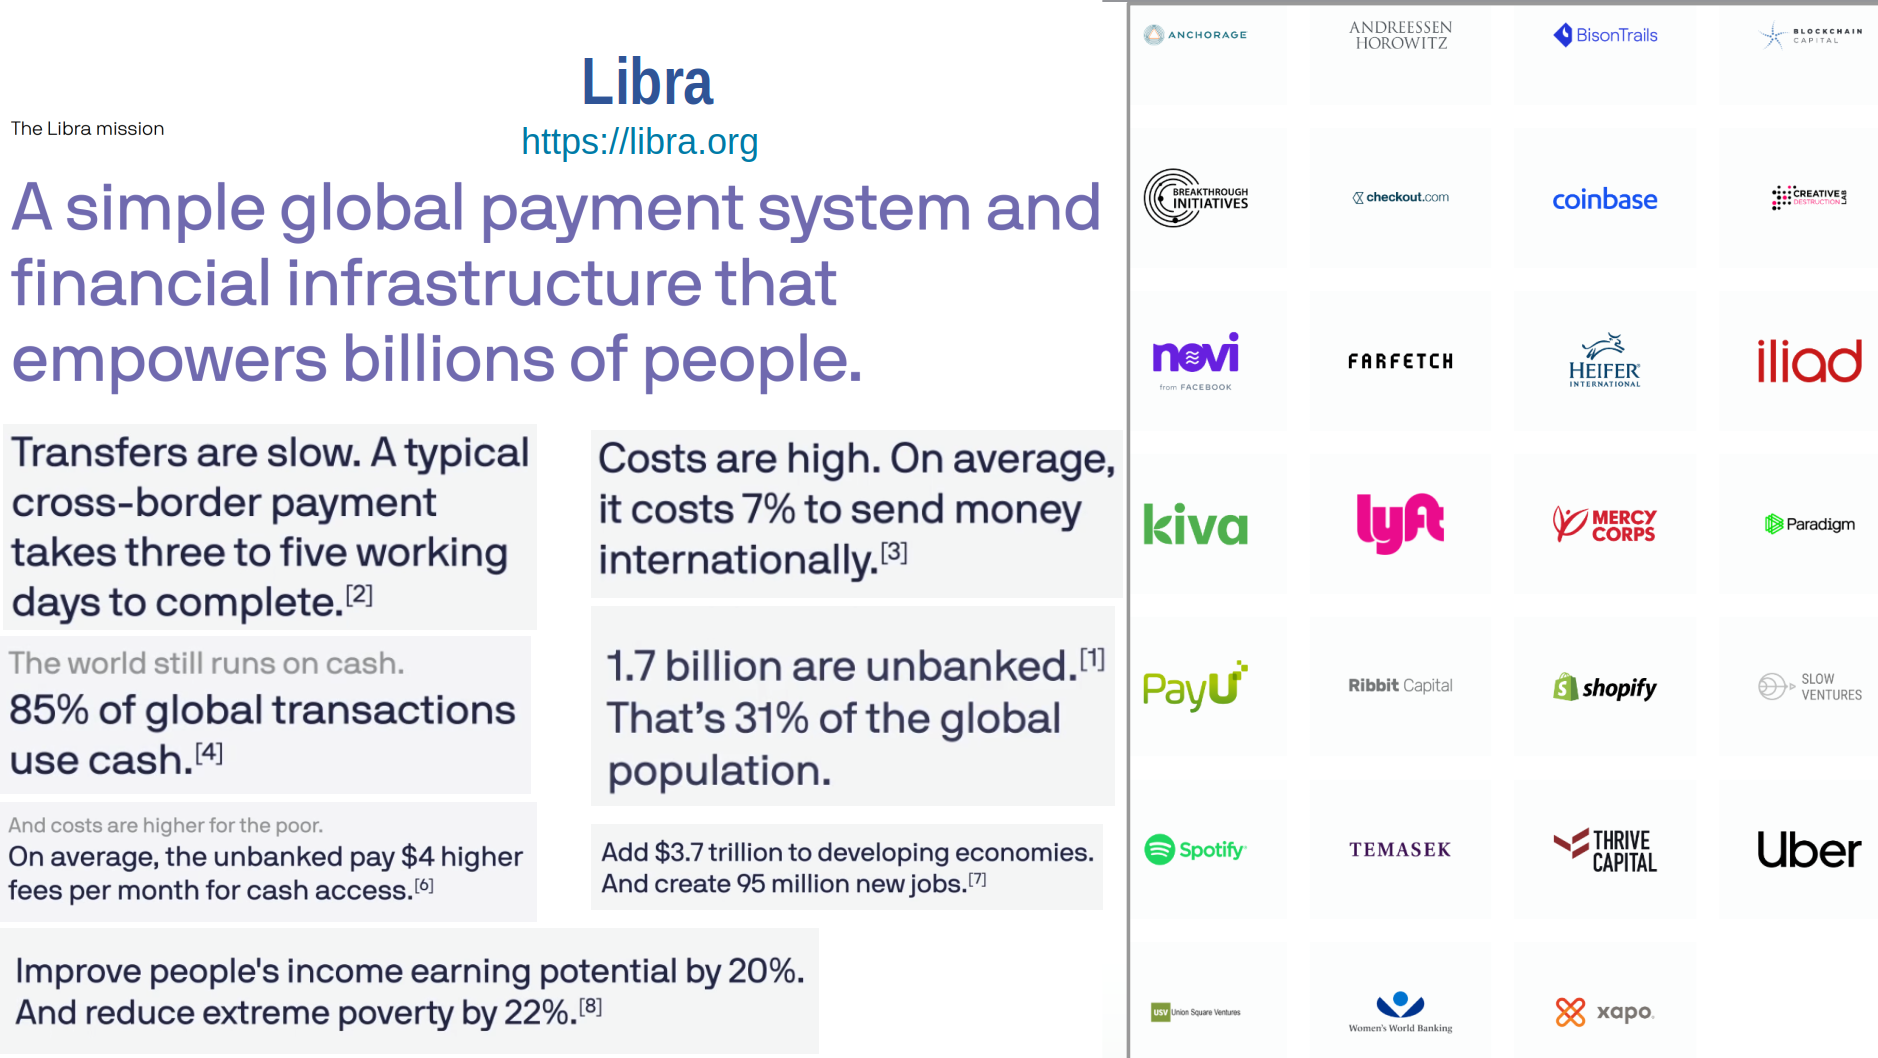
\includegraphics[height=6.5cm]{../pics/central_banks/libra-2020}
	\end{figure}
}

%----------------------------------------------------------------------------
\subsection{The response of central banks}
\frame{
  \frametitle{The allergic response of central banks}
	\begin{figure}
        \centering
		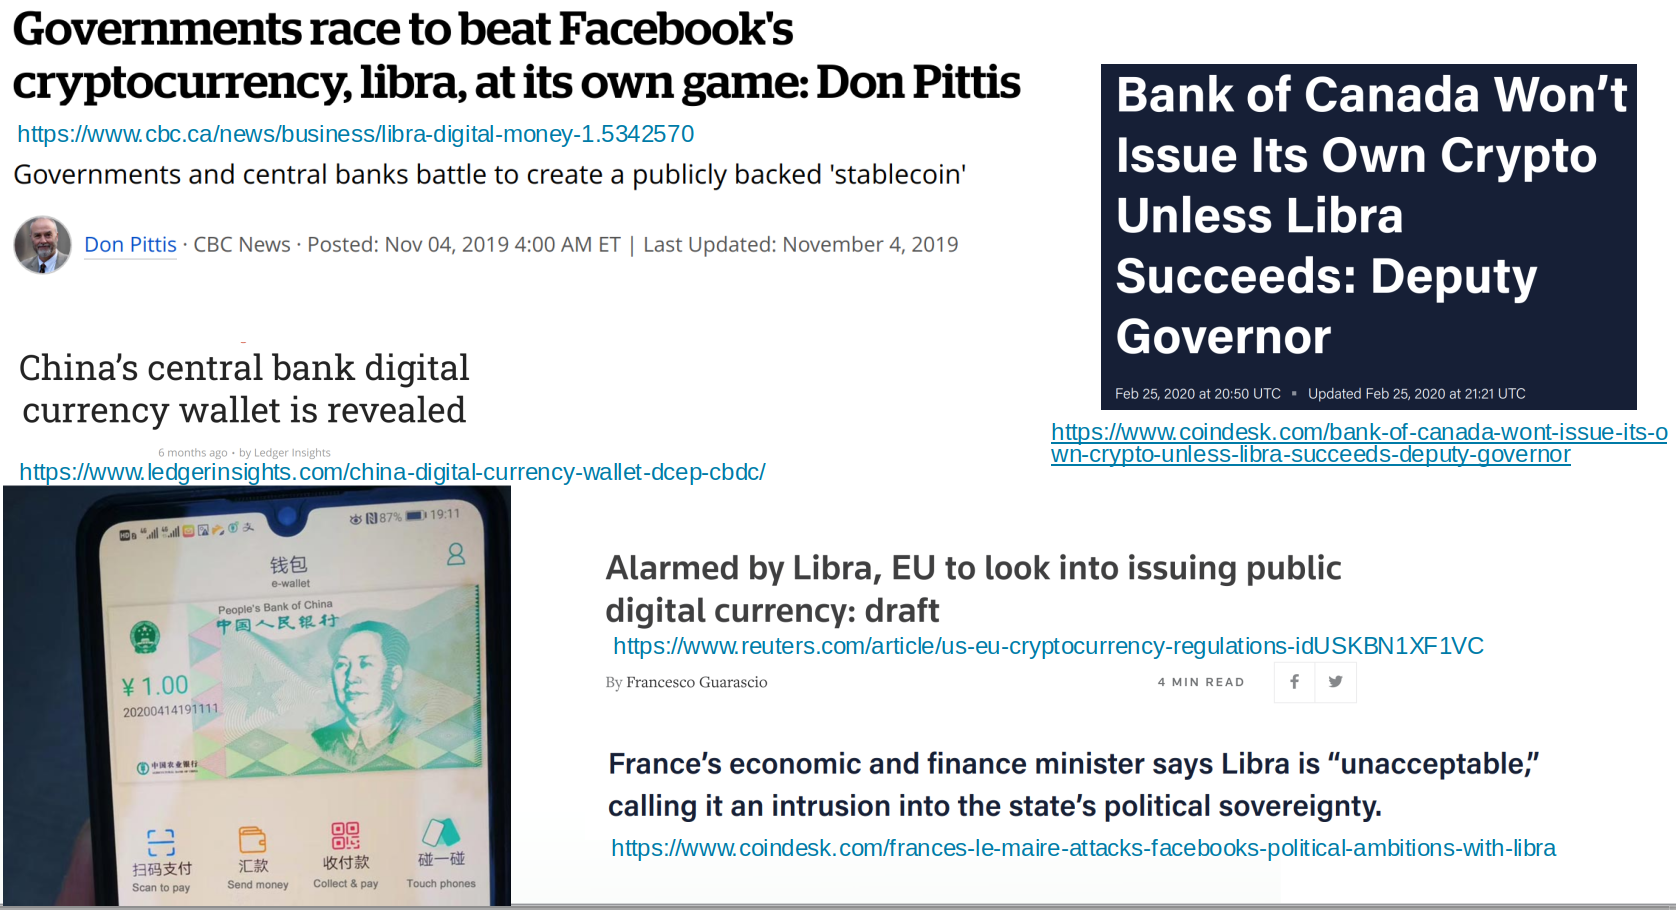
\includegraphics[height=6.5cm]{../pics/central_banks/libra-response-2020}
	\end{figure}
}

\frame{
    \frametitle{Value proposition}
    \textbf{At first it looked like a joke}. Bitcoin is the first alternative to the world banking system, carrying an anarchist and Cyberpunk mindset.\\
    \vspace{1em}
    \textbf{Then a big scare}. Libra is another alternative, proposed by large American power houses (mainly Facebook).\\
    \vspace{1em}
    \textbf{Can countries maintain control on their fiat money?}
}

\frame{
    \frametitle{Central Banks have been slowly studying the pace}
    Christine Lagarde (former head of the IMF and now at the ECB) has been keen to the use of Blockchain by central banks (\citeyear{lagarde2017}).
    The IMF has published a staff discussion note on the topic of Central Bank Digital Currencies (\citeyear{imf2018:cbdc}).\\
    \vspace{1em}
    Potential benefits:
    \begin{itemize}
        \item financial inclusion
        \item security and consumer protection
        \item privacy
    \end{itemize}
    \vspace{1em}
    Obviously, there are also risks for central banks: loss of control on currency, inability to remain the lender of last resort\ldots 
}

\frame{
	\frametitle{The Bank of Canada}
	\begin{figure}
        \centering
		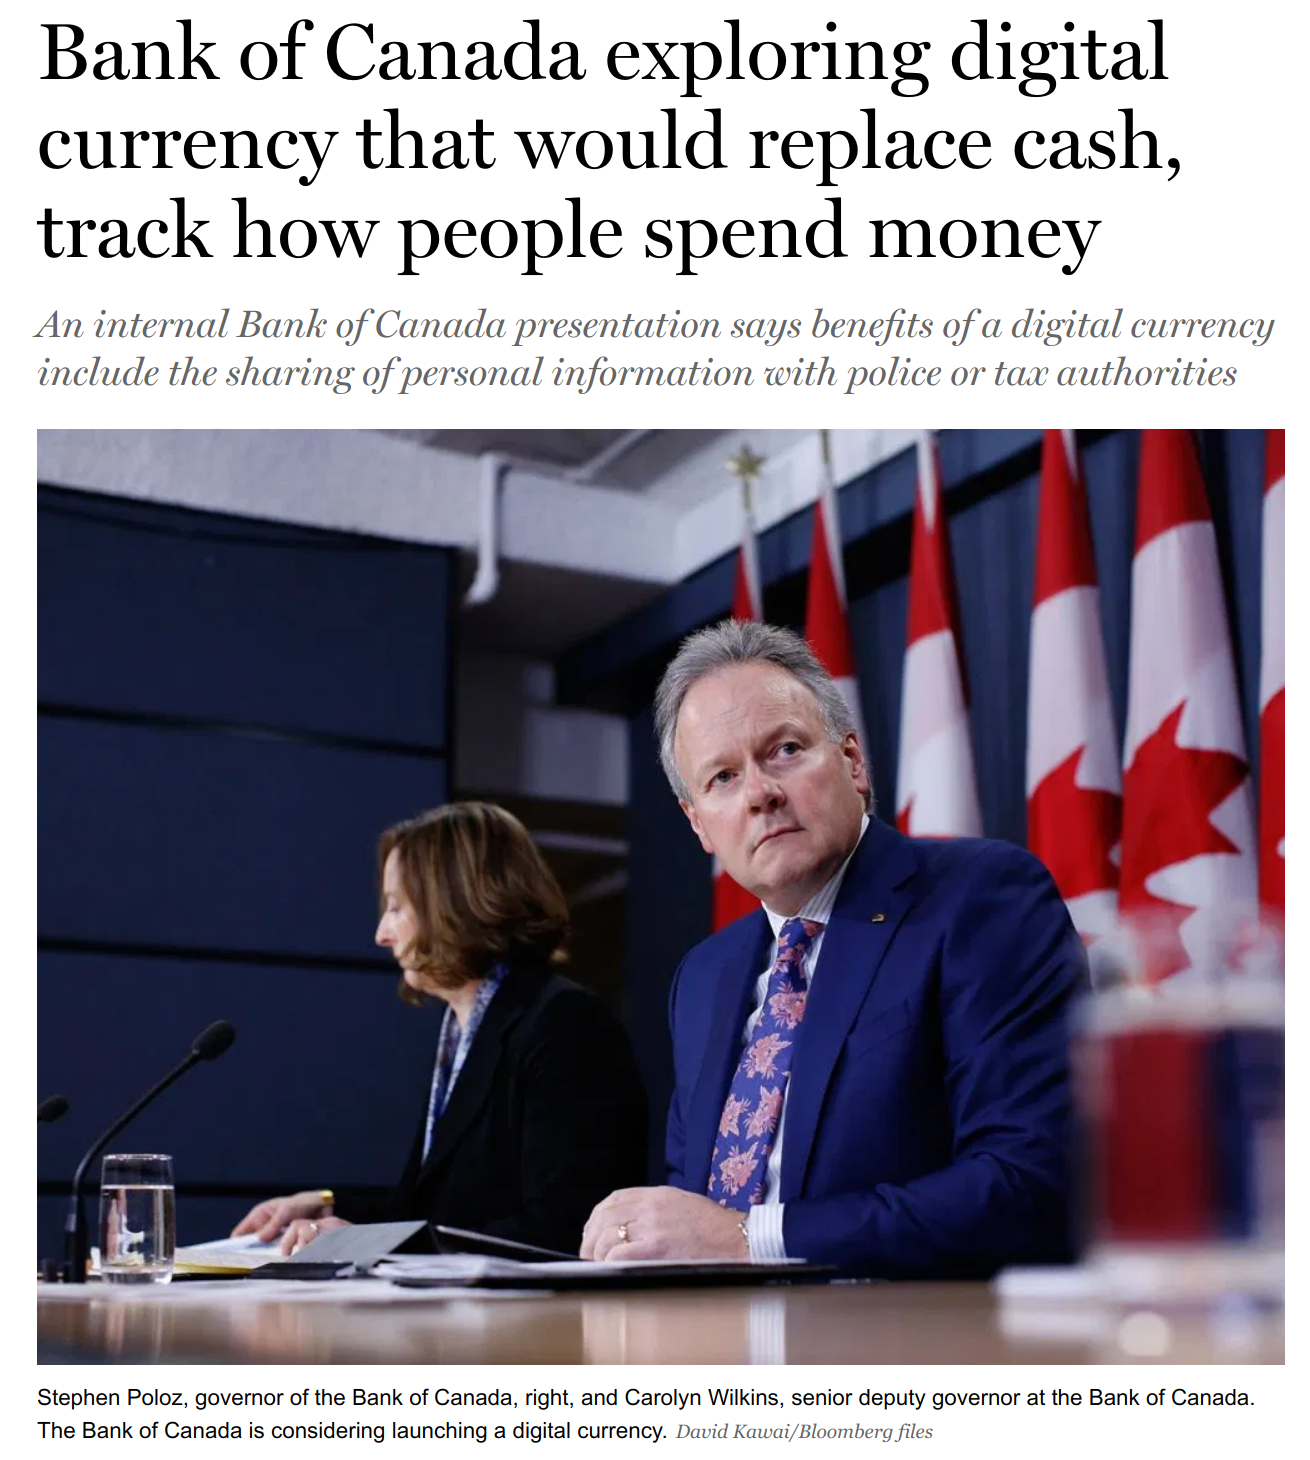
\includegraphics[height=5.5cm]{../pics/cryptocurrency/financialpost-bankofcanada-crypto2019}
        \caption{\cite{financialpost2019:bankofcandacrypto}}
%        \caption{\url{https://business.financialpost.com/technology/blockchain/bank-of-canada-exploring-digital-currency-that-would-replace-cash-track-how-people-spend-money}}
	\end{figure}
    The Bank of Canada has explored the digital currency space since 2012.
    Current discussion involves sharing information with law enforcement and tax authorities.
}

\frame{
  \frametitle{Central Bank Digital Currency (CBDC) models}
	\begin{figure}
        \centering
		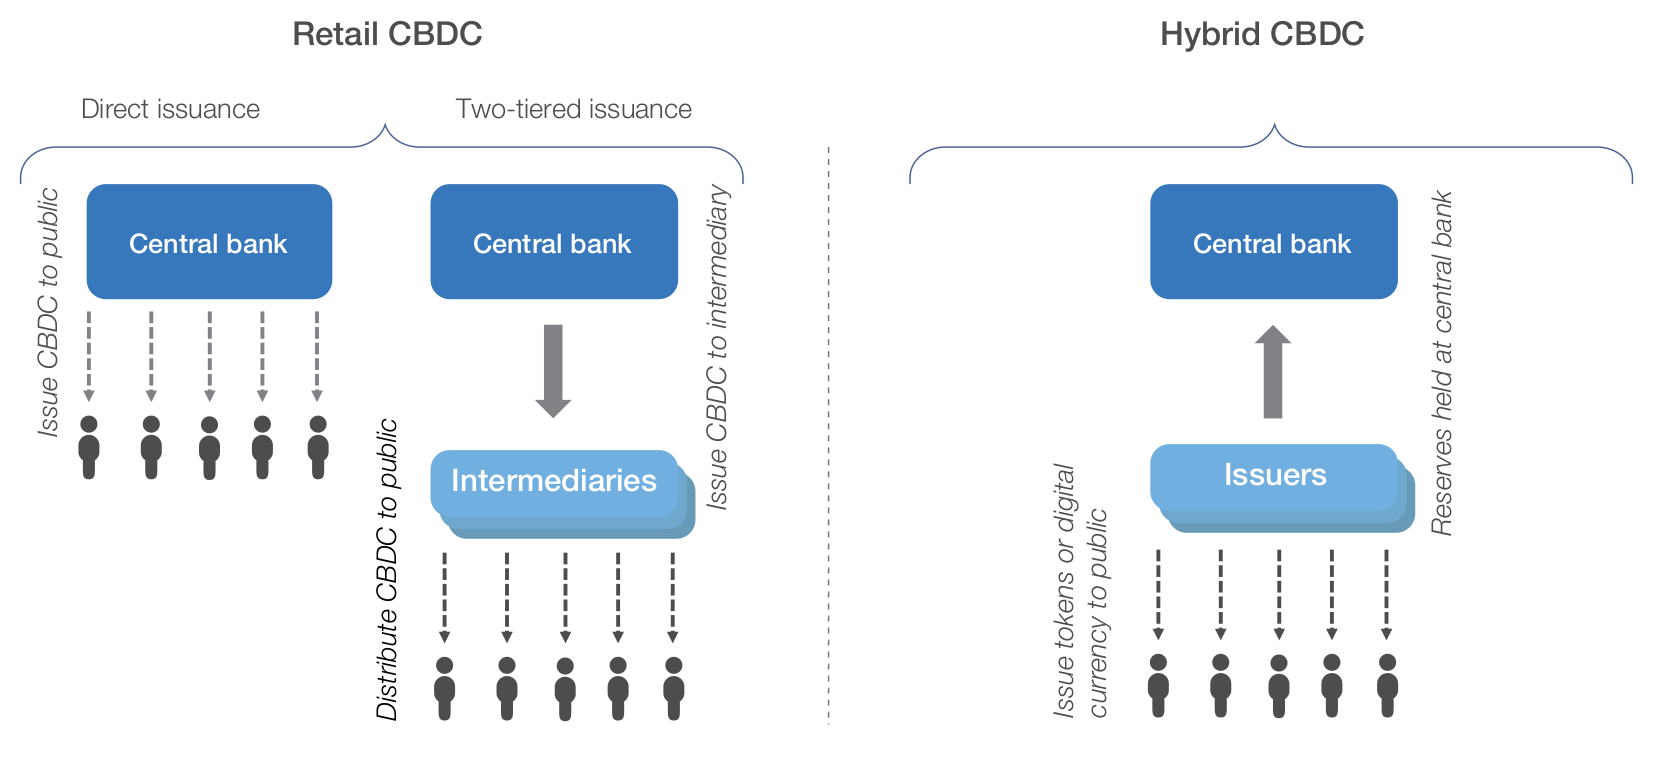
\includegraphics[width=11cm]{../pics/central_banks/cbdc-models}
	\end{figure}
}

\frame{
    \frametitle{Key drivers}
    \begin{itemize}
    \item Sovereignty (e.g. fiscal policy, monetary policy)
    \item A CBDC allows greater control including monitoring all transactions, sharing information with police and tax authorities, helicopter money (e.g. COVID rescue package such as CERB), programmable money
    \item Hegemony of the US dollar (including an alternative to SWIFT)
    \item Rising debt -the Great reset
    \item Cantillon effect
    \end{itemize}
}

\frame{
  \frametitle{Status at the People Bank of China (PBOC)}
	\begin{figure}
        \centering
		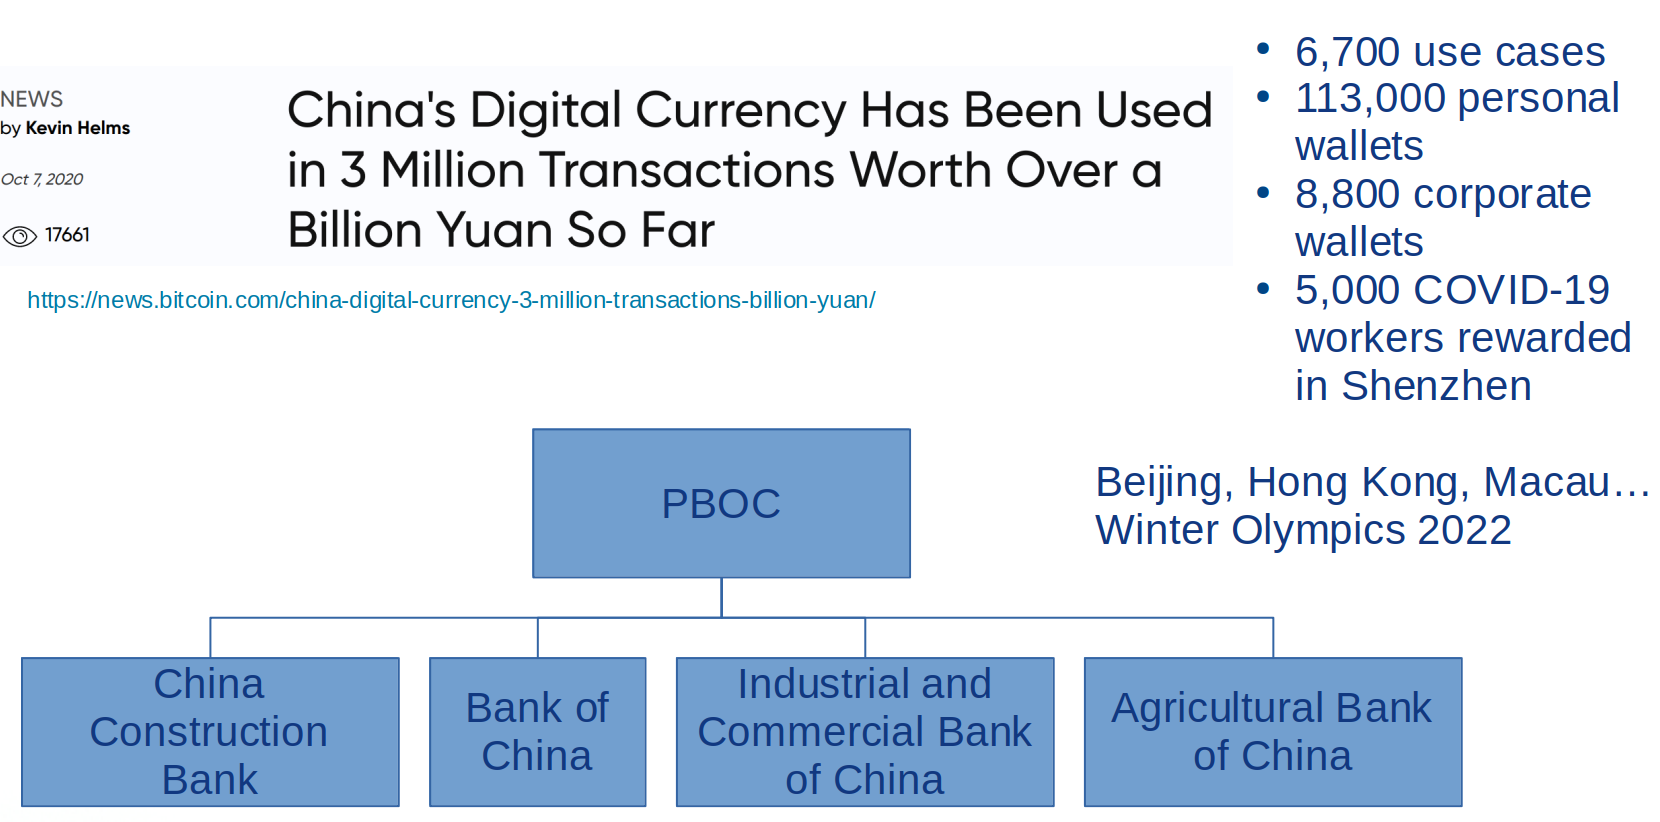
\includegraphics[width=11cm]{../pics/central_banks/pboc-2020}
	\end{figure}
}

\frame{
  \frametitle{The Bank of Canada (Feb 2020 update)}
	\begin{figure}
        \centering
		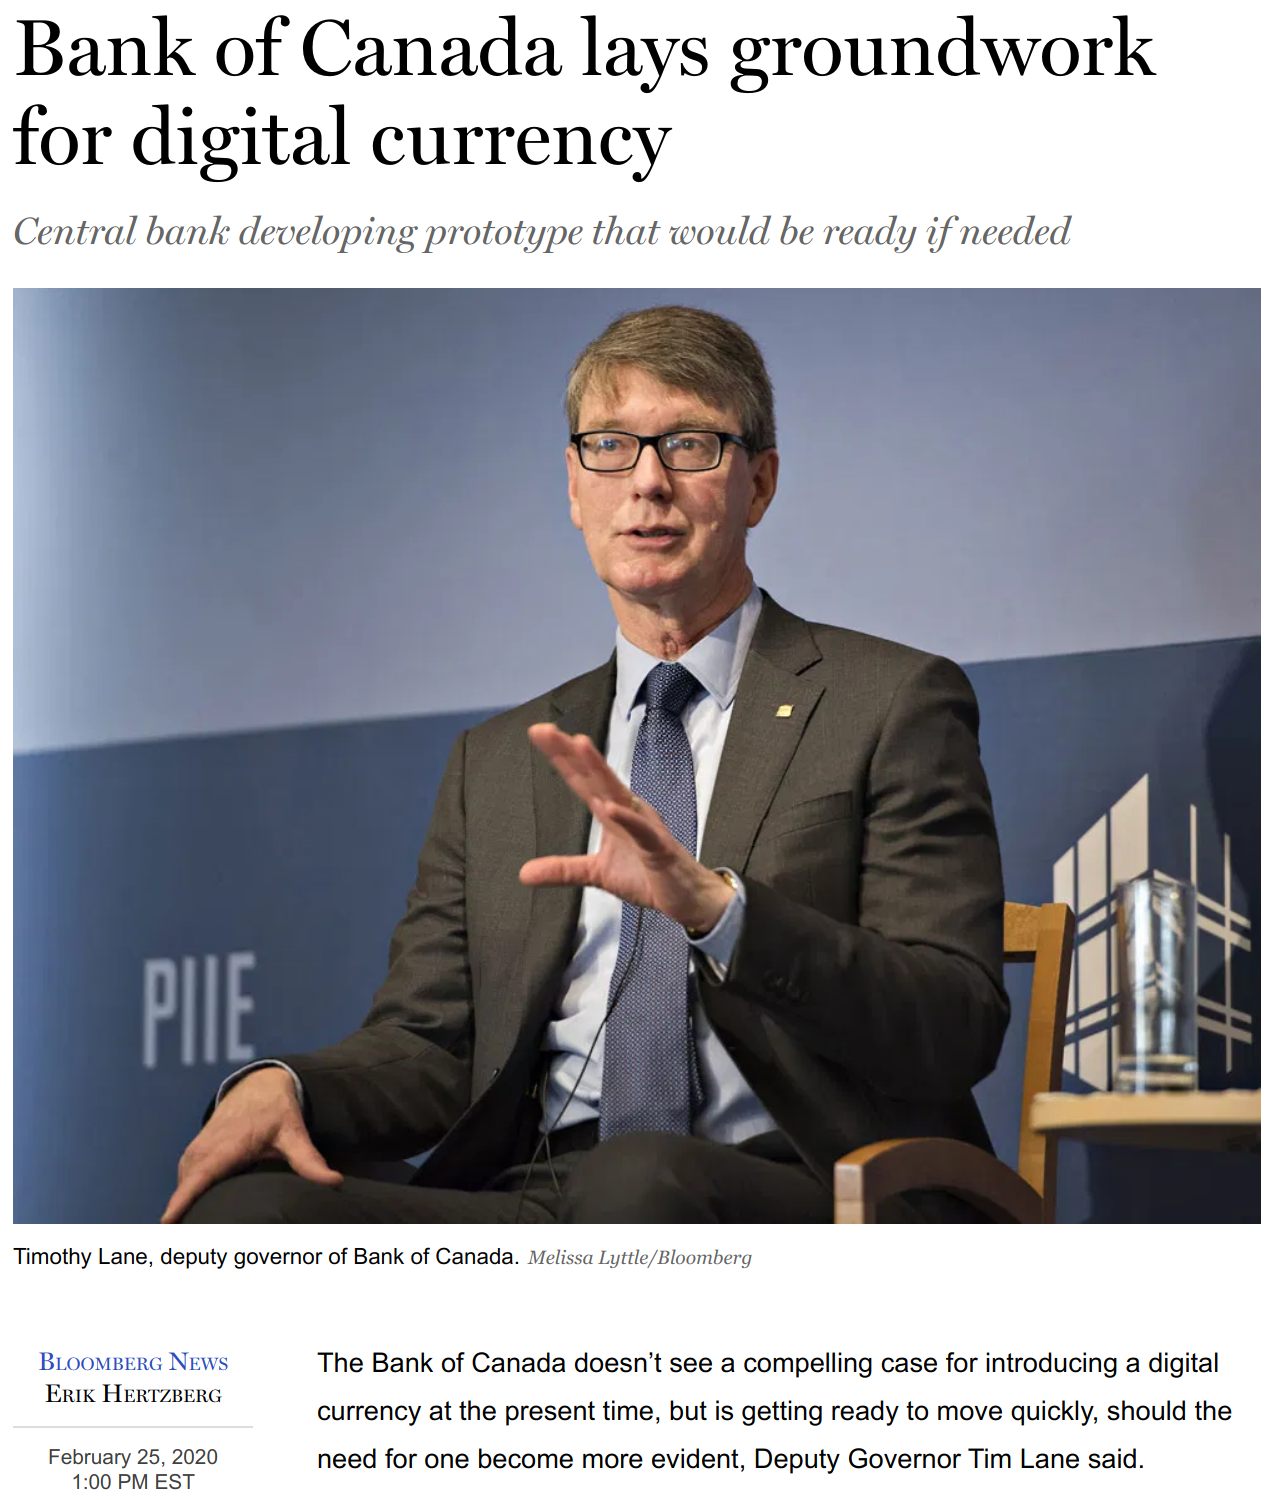
\includegraphics[height=6.5cm]{../pics/cryptocurrency/fp2020-02-boc}
        \caption{\cite{financialpost2020:bankofcandacrypto}}
	\end{figure}
}

\frame{
  \frametitle{Six central banks to collaborate on digital currency research}
	\begin{figure}
        \centering
		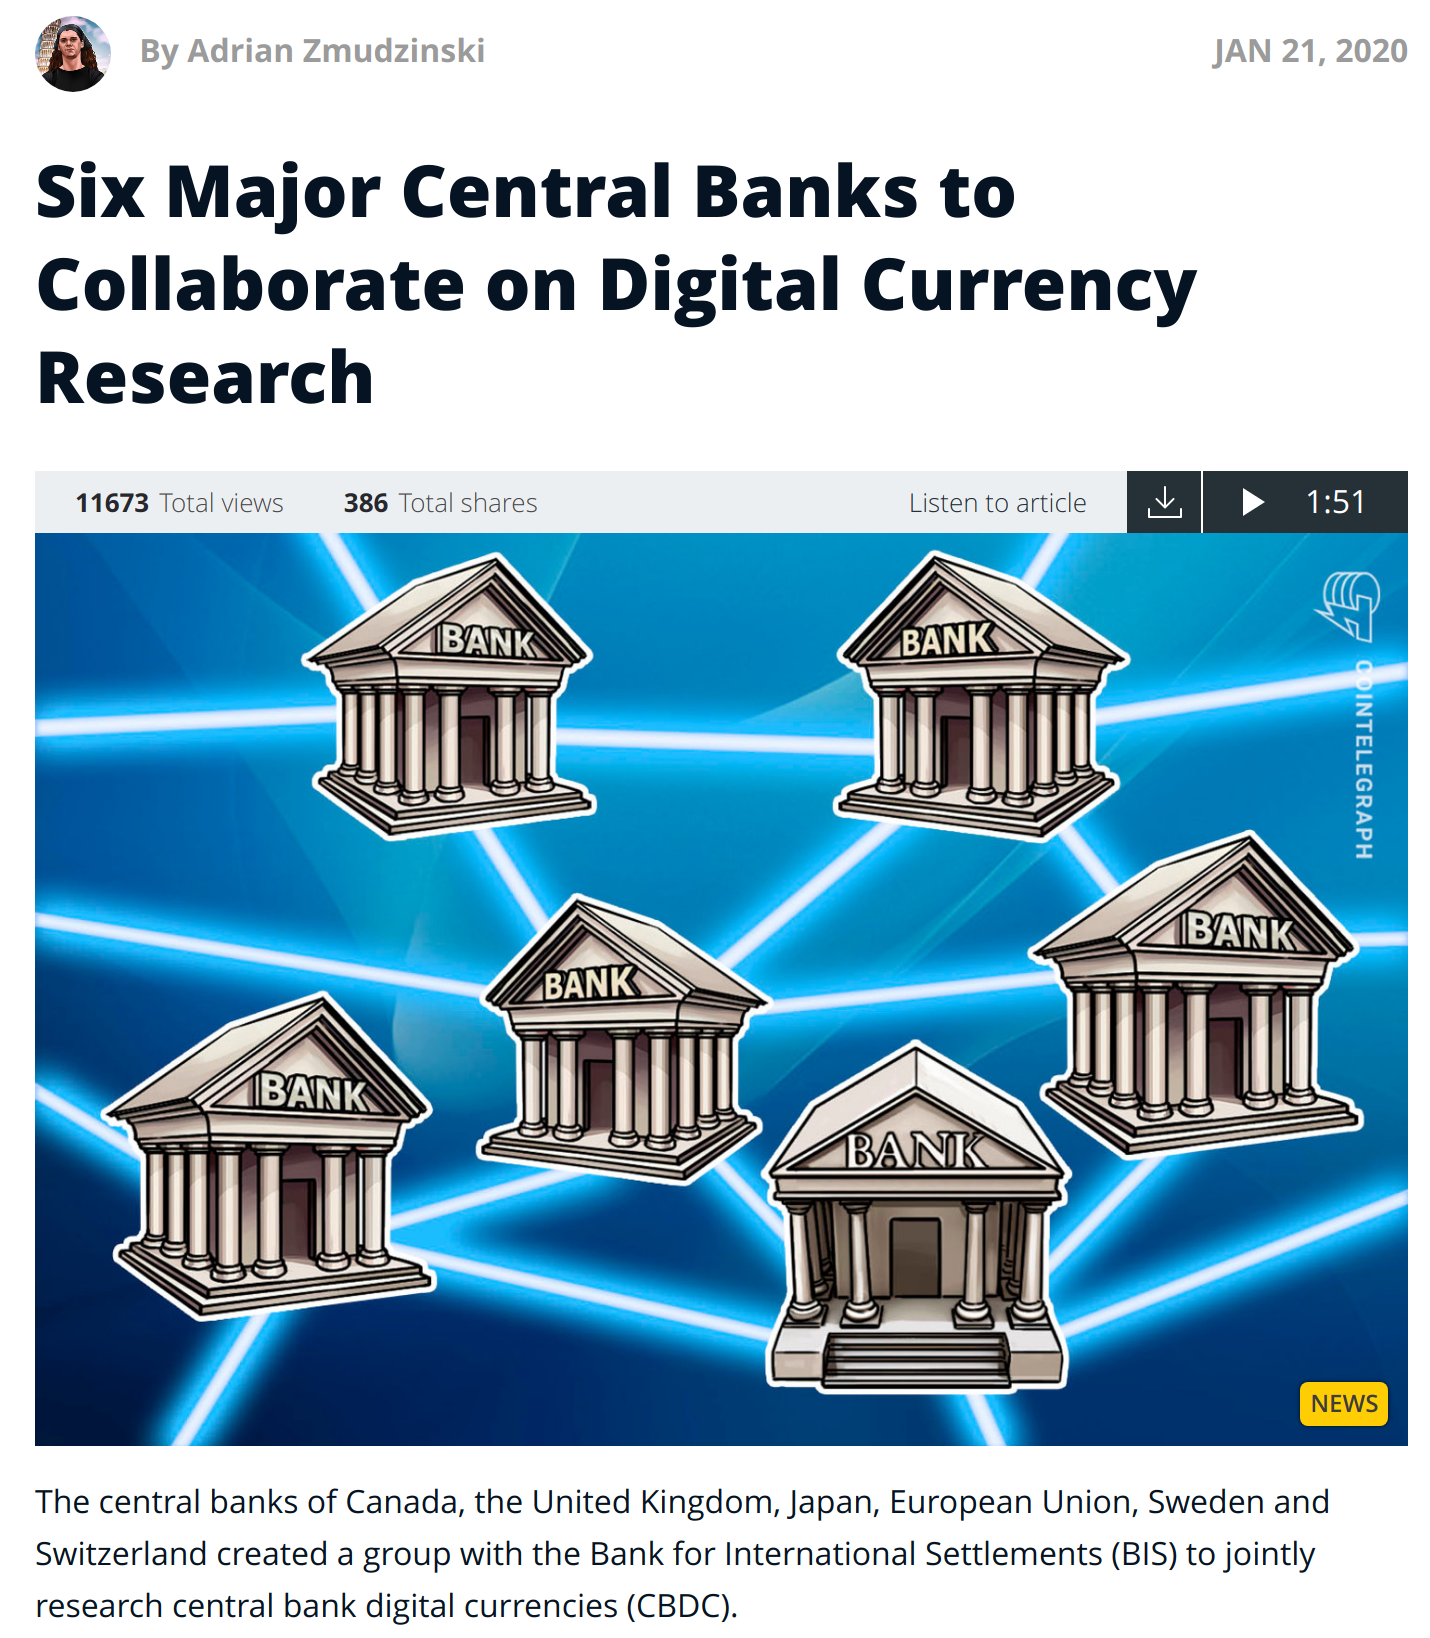
\includegraphics[height=5.5cm]{../pics/cryptocurrency/cointelegraph-2020-01-bis}
        \caption{\cite{cointelegraph:bis}}
	\end{figure}
  ``The central banks of Canada, the United Kingdom, Japan, European Union, Sweden and Switzerland created a group with the Bank for International Settlements (BIS) to jointly research central bank digital currencies (CBDC).''
}

\frame{
  \frametitle{Coordination if not Standardization}
	\begin{figure}
        \centering
		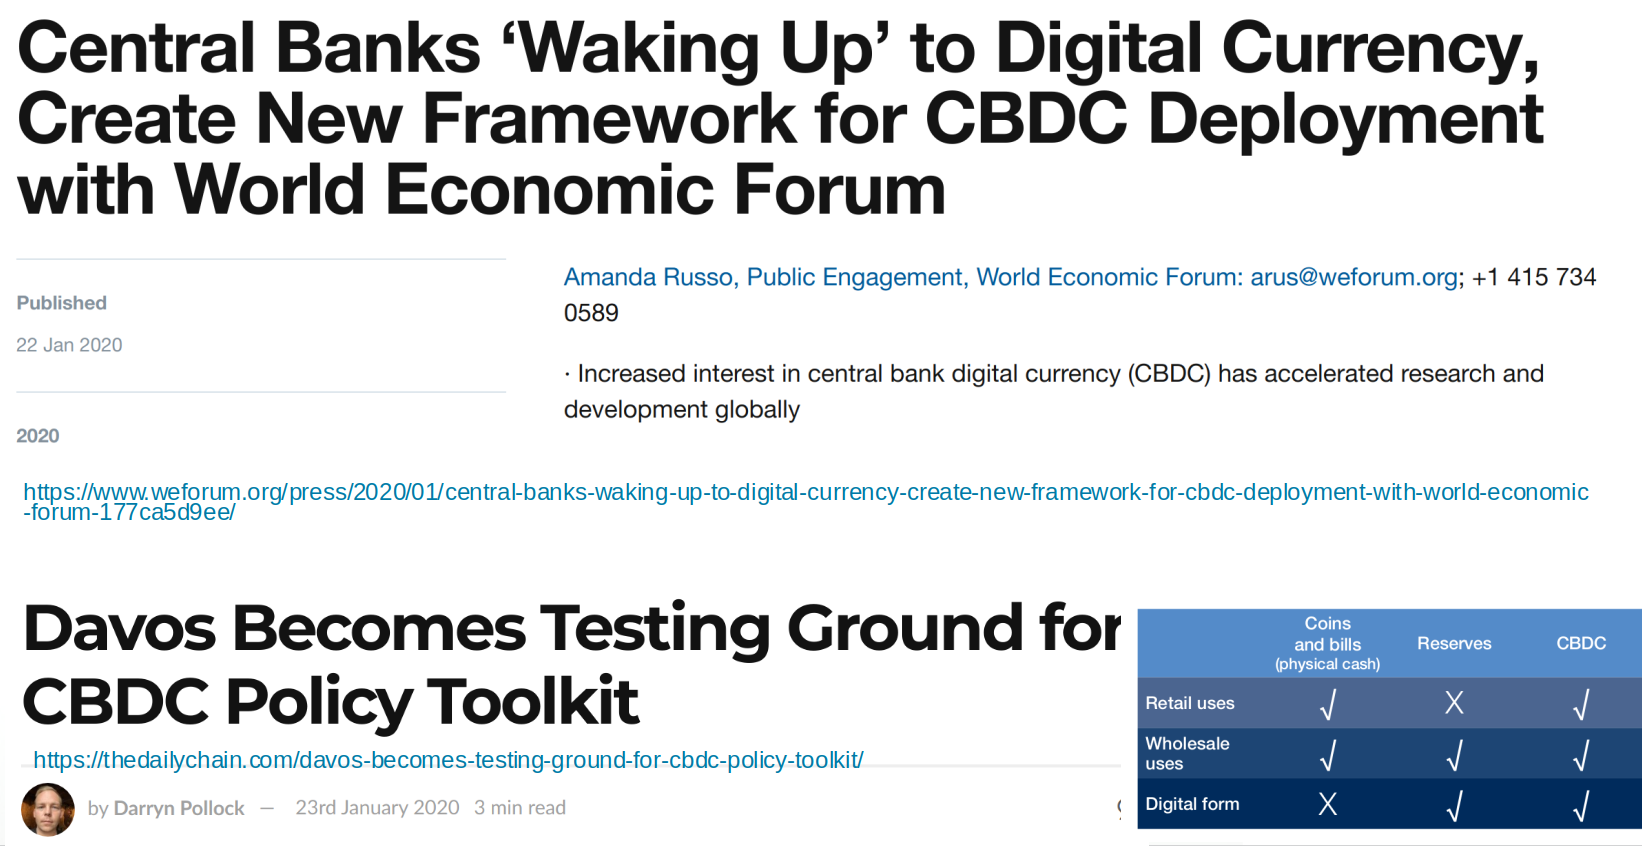
\includegraphics[height=6.5cm]{../pics/central_banks/central-banks-davos}
	\end{figure}
}


%\frame{
%	\frametitle{The People's Bank of China}
%	\begin{figure}
%        \centering
%		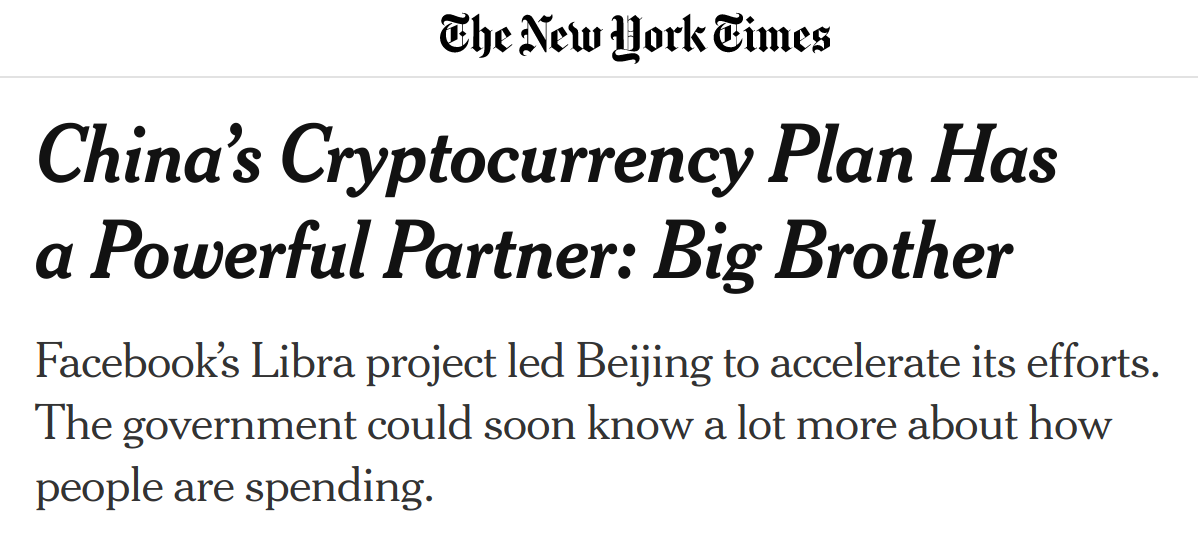
\includegraphics[width=11.5cm]{../pics/cryptocurrency/nytimes2019-china-crypto}
%        \caption{\cite{nytimes2019:china-crypto}}
%        \caption{\url{https://www.nytimes.com/2019/10/18/technology/china-cryptocurrency-facebook-libra.html}}
%	\end{figure}
%    See also \citeauthor{forbes201908:chinacrypto}'s article in Forbes (\citeyear{forbes201908:chinacrypto}).
%% also check   https://www.forbes.com/sites/michaeldelcastillo/2019/08/27/alibaba-tencent-five-others-to-recieve-first-chinese-government-cryptocurrency/#1fb606111a51
%% "In addition to preventing regional banks and other organizations from being disintermediated, Mu said the two-tiered system is designed to “curb” public demand for other %cryptographic assets, consolidate China’s national currency sovereignty, ensure that the central bank maintains control over monetary policy affecting the currency, increase the %likelihood of people using the currency, distribute the risk of having all the authority directly in the hands of the central bank and encourage competition between the organizations %that receive the cryptocurrency."
%}

\frame{
    \frametitle{Project and countries of interest}
    \begin{itemize}
        \item Libra and Calibra
        \item R3 Corda (e.g. Project Jasper, MAS)
        \item Ethereum (e.g. France, MAS)
        \item Stellar (e.g. Ukraine)
        \item Tezos (e.g. France, Ukraine)
    \end{itemize}
}


%----------------------------------------------------------------------------
%\subsection{Crypto alternatives}

\frame{
    \frametitle{The interesting case of Basis: an algorithmic central bank}
    Basis (formerly Basecoin) was proposed as a stable coin relying on algorithms.
    The coin could be pegged to any asset or basket of assets.\\
    \vspace{1em}
    The project, the first from Intangible Labs, boasts investors including 1confirmation, Andreessen Horowitz, Bain Capital Ventures, Digital Currency Group, MetaStable Capital, Pantera Capital and PolyChain Capital.\\
    \vspace{1em}
    In June 2017, there were only a handful of stable coins (Tether, BitShares/BitUSD). Maker DAO would issue its white paper later, in the last month of 2017.
    Today, more than 50 stable coins have been identified (\citeauthor{alyzesam2019:completeguidestablecoins}, \citeyear{alyzesam2019:completeguidestablecoins}).\\
% https://blog.bitmex.com/a-brief-history-of-stablecoins-part-1/
% https://hackernoon.com/2019-complete-stablecoin-guide-0n9es3zab
    \vspace{1em}
    The Basis white paper (\citeyear{basis:whitepaper}) is available at \url{https://www.basis.io/basis_whitepaper_en.pdf}
}

\frame{
    \frametitle{The vision: an autonomous and decentralized central bank}
    \begin{exampleblock}{From the white paper}
    ``Basecoin would present the world with both the technology and the opportunity to develop an independent, transparent and potentially more stable monetary policy than anything that’s ever been possible via central bank''
    \end{exampleblock}
}

\frame{
    \frametitle{The team}
    \begin{itemize}
        \item Nader Al-Naji, ex Software Engineer at Google, Princeton Computer Science and Maths
        \item Lawrence Diao, ex Software Engineer at Google, Princeton Computer Science Summa Cum Laude
        \item Josh Chen, ex machine learning engineer, Princeton Computer Science Summa Cum Laude
        \item Susan Sidd, ex Managing Director and Legal Director at Goldman Sachs, JD from Harvard
        \item and other \url{https://www.basis.io/\#team}
    \end{itemize}
}


\frame{
    \frametitle{The technology}
    Basis is not backed by fiat or cryptocurrencies. It relies on \href{https://en.wikipedia.org/wiki/Seigniorage}{Seigniorage} (and \href{https://en.wikipedia.org/wiki/Demurrage\_(currency)}{Demurrage}) principles and algorithms.\\
    \vspace{1em}
    %Basis remains stable by incentivizing traders to buy and sell Basis in response to changes in demand. These incentives are set up through regular, on-chain auctions of “bond” and “share” tokens, which serve to adjust Basis supply.
    The protocol would watch indices (e.g. US Dollar). Like a central bank applying the Quantity theory of money (QTM), a smart contract would leverage oracles to contract or expand its token supply to control its token value (e.g. exchange rate with the US Dollar). When the price of Basis is too high, it would mint tokens (``print'' money) to give it to token holders. When the price of Basis is too low, it would trigger a bond sale at a discount to take coins out of circulation.\\
    \vspace{1em}
    Three tokens:
    \begin{itemize}
    \item basecoin is the first token considered, pegged to 1 USD
    \item base bonds used to managed the volatility of basecoin
    \item base shares idem
    \end{itemize}
}





% ======================================================================================================
%                         Other usecases 
% ======================================================================================================
\section{Other usecases}
 \frame{
	\frametitle{A Token can represent anything}
	\begin{figure}
		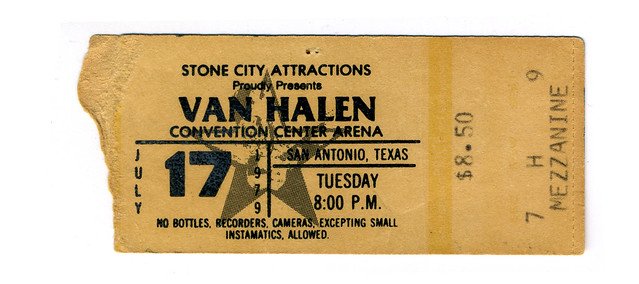
\includegraphics[width=11cm]{../pics/tokenization/ticket-van-halen}
		\captionsetup{justification=centering}
		\caption{Credit~: \href{https://www.flickr.com/photos/hmk/2121424630}{H. Michael Karshis}}
	\end{figure}
}

\frame{
	\frametitle{Native Currency}
	\begin{figure}
		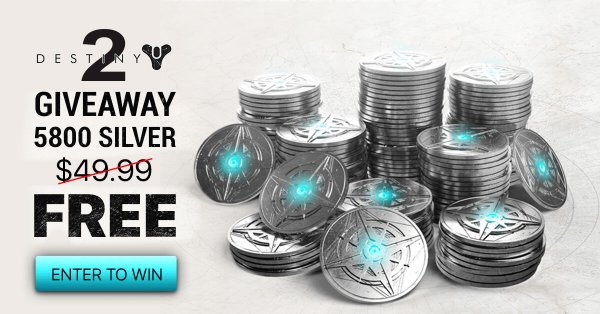
\includegraphics[height=6cm]{../pics/tokenization/destiny-silver}
		\captionsetup{justification=centering}
		\caption{Source~: give.zone (also sold on Amazon, PlayStation store, etc)}
	\end{figure}
}

\frame{
	\frametitle{Case Study: Gold tokenization}
	\begin{figure}
		
\includegraphics[height=3cm]{../pics/tokenization/640px-Gold_bullion_bars}
		\captionsetup{justification=centering}
		\caption{Credit~: \href{https://commons.wikimedia.org/wiki/File:Gold_bullion_bars.jpg}{stevebidmead}}
	\end{figure}
	\begin{itemize}
		\item JP Morgan tokenizes Gold (\cite{thetokenist2019:jpmorgangold})
		\item LAToken partners with MyGold (\cite{latoken2017:gold})
		\item \ldots 
	\end{itemize}
}

\frame{
	\frametitle{Case Studies: fractional real estate and track \& trace (Tuna)}
	\begin{figure}
		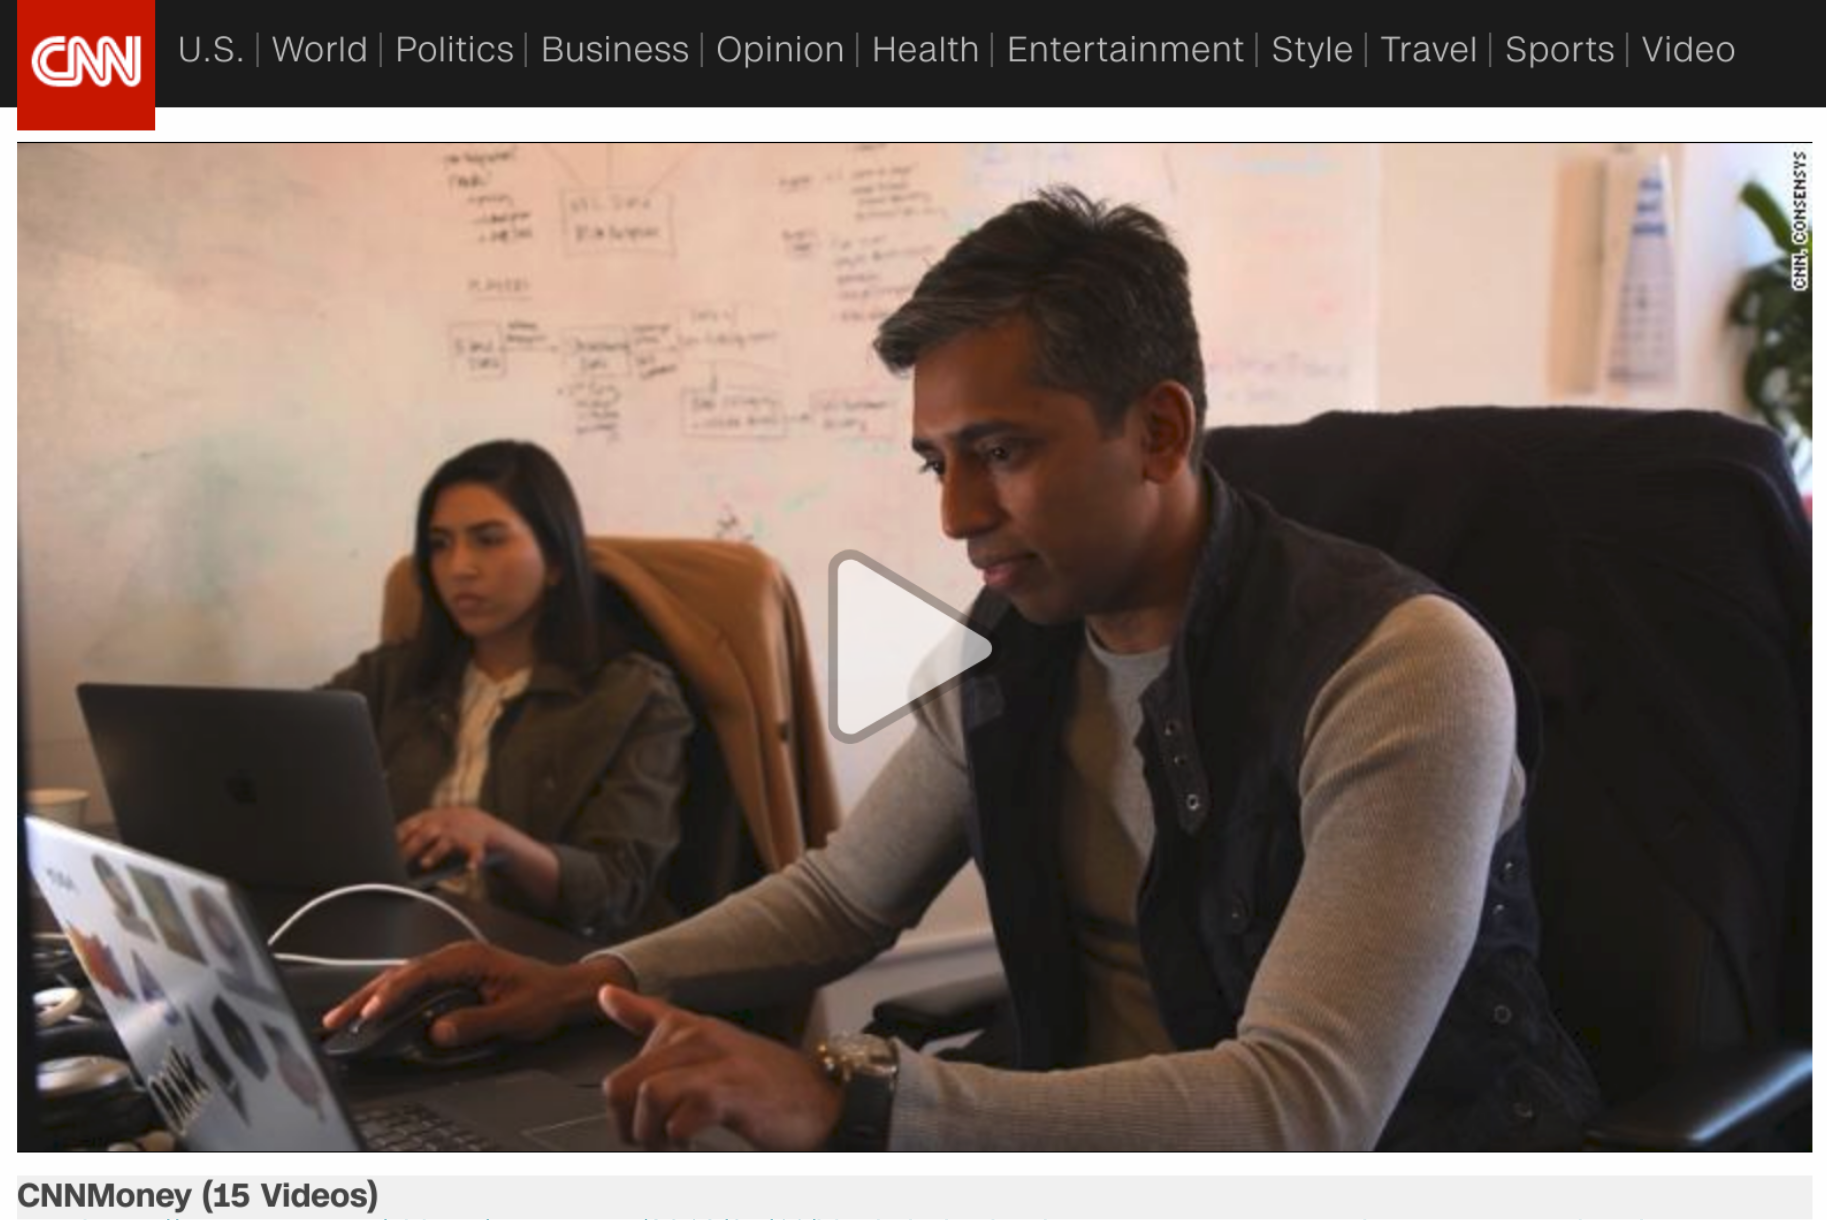
\includegraphics[height=6cm]{../pics/ConsenSys/case_studies/cnn2018-viant-meridio}
		\captionsetup{justification=centering}
		\caption{Source~: \cite{cnn2018:viant-meridio}}
	\end{figure}
}

\frame{
	\frametitle{Use Cases in Media \& Entertainment}
	\begin{figure}
		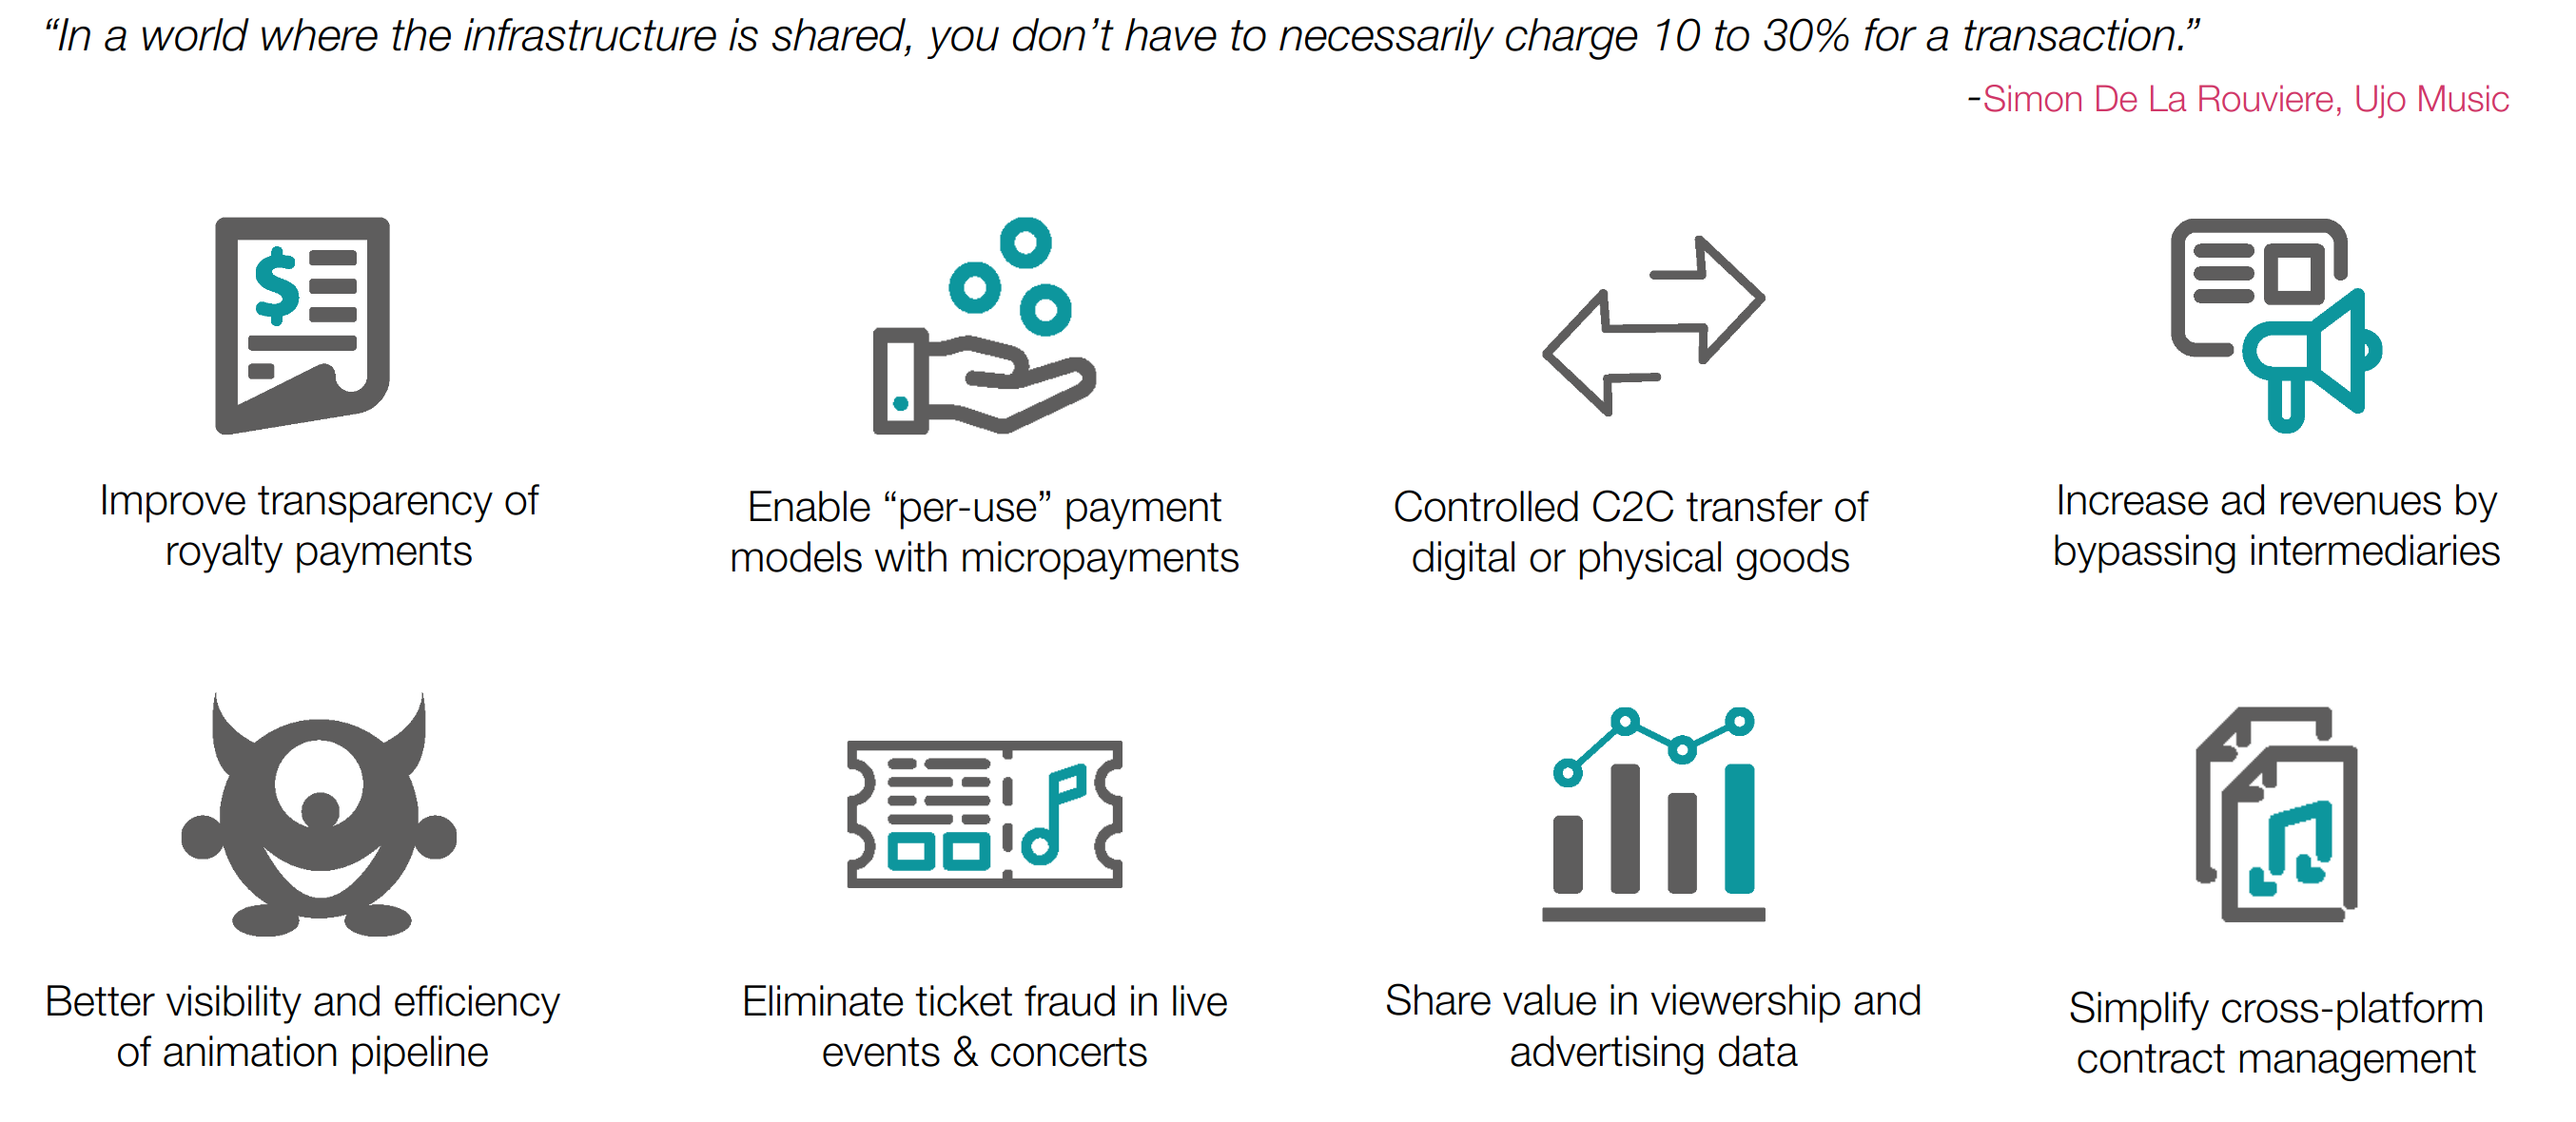
\includegraphics[width=11cm]{../pics/ConsenSys/industry/use-case-ME}
	\end{figure}
}

\frame{
	\frametitle{In Toronto: Prescient is developing an Attribution Ledger for Work of Arts}	
	\begin{figure}
		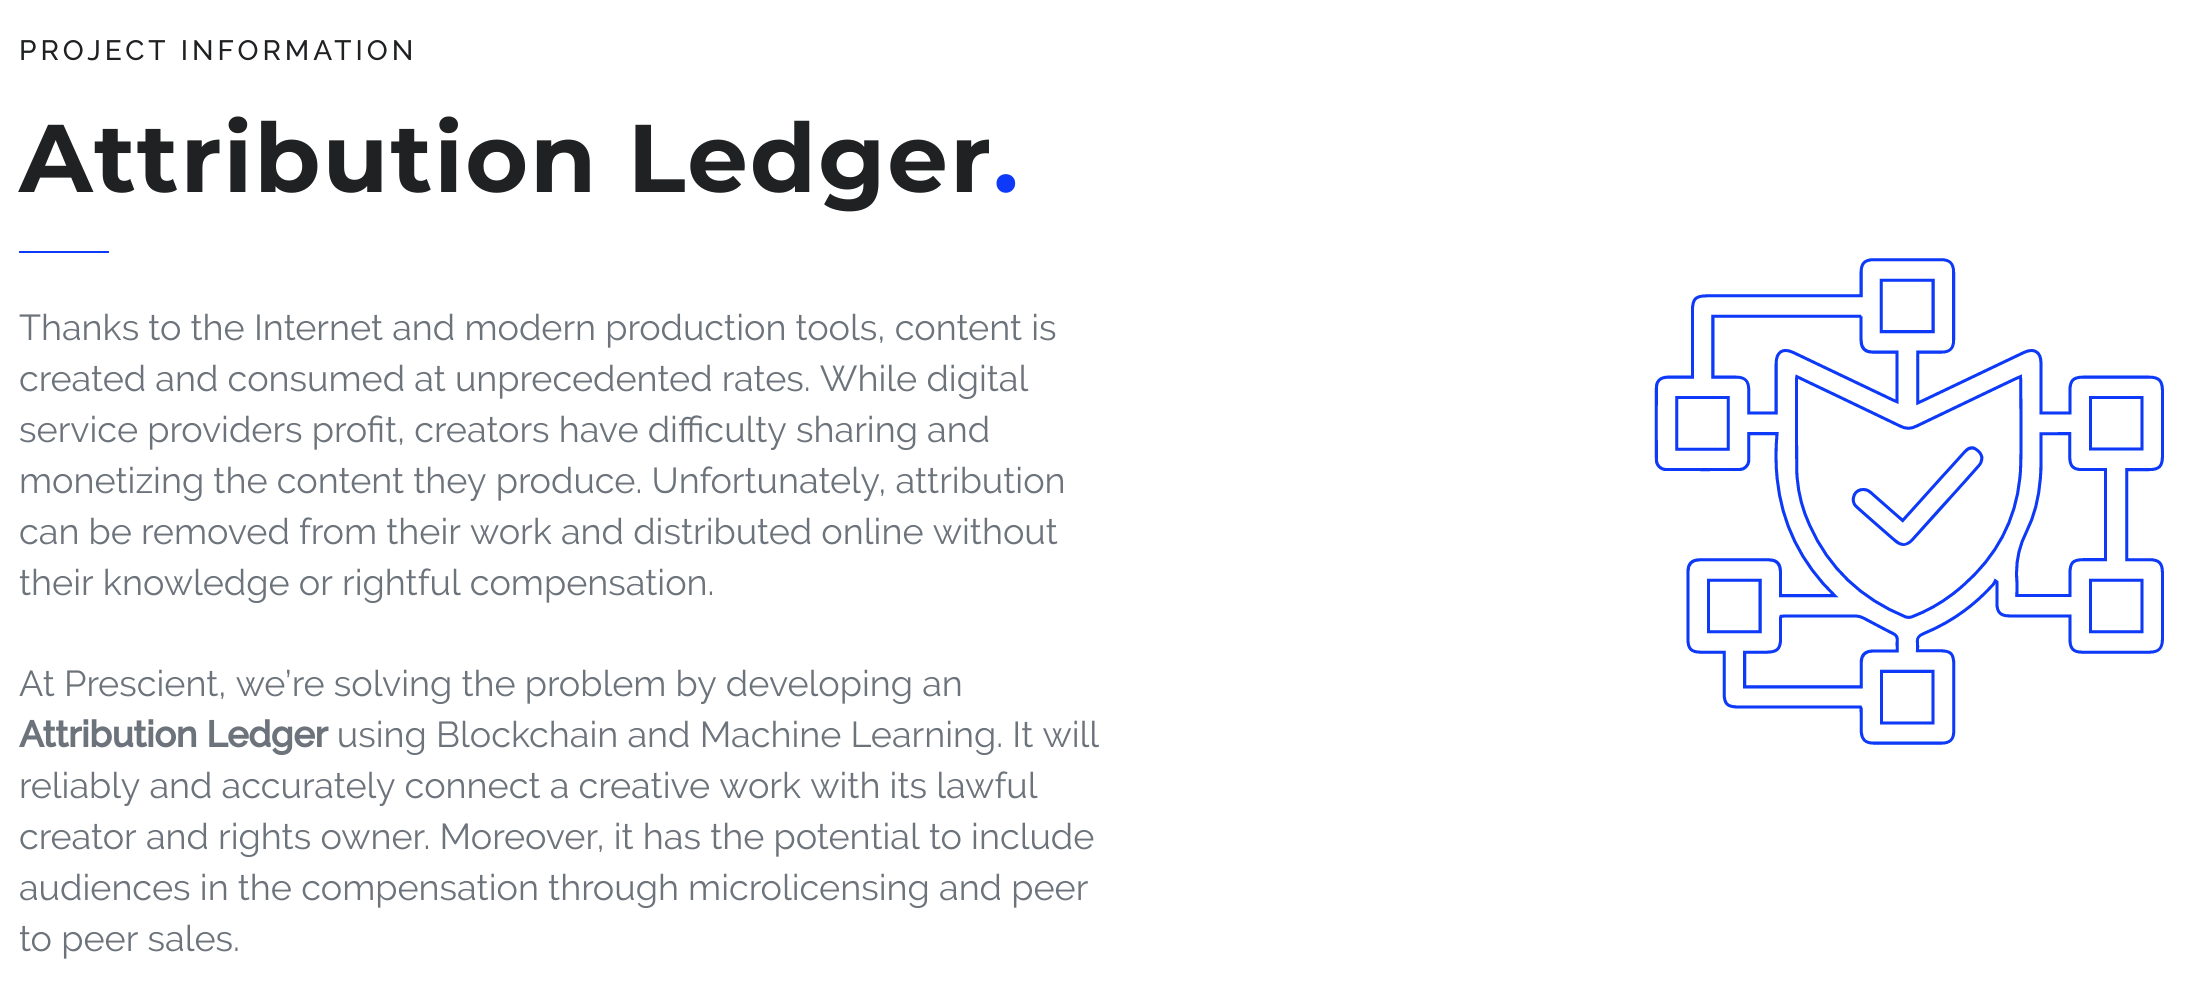
\includegraphics[width=11cm]{../pics/tokenization/prescient-attribution-ledger}
		\captionsetup{justification=centering}
		\caption{Source~: \url{https://prescientinnovations.com/attribution-ledger}}
	\end{figure}
}

\begin{frame}   
	\frametitle{Case study: Baoquan}
	\begin{figure}
		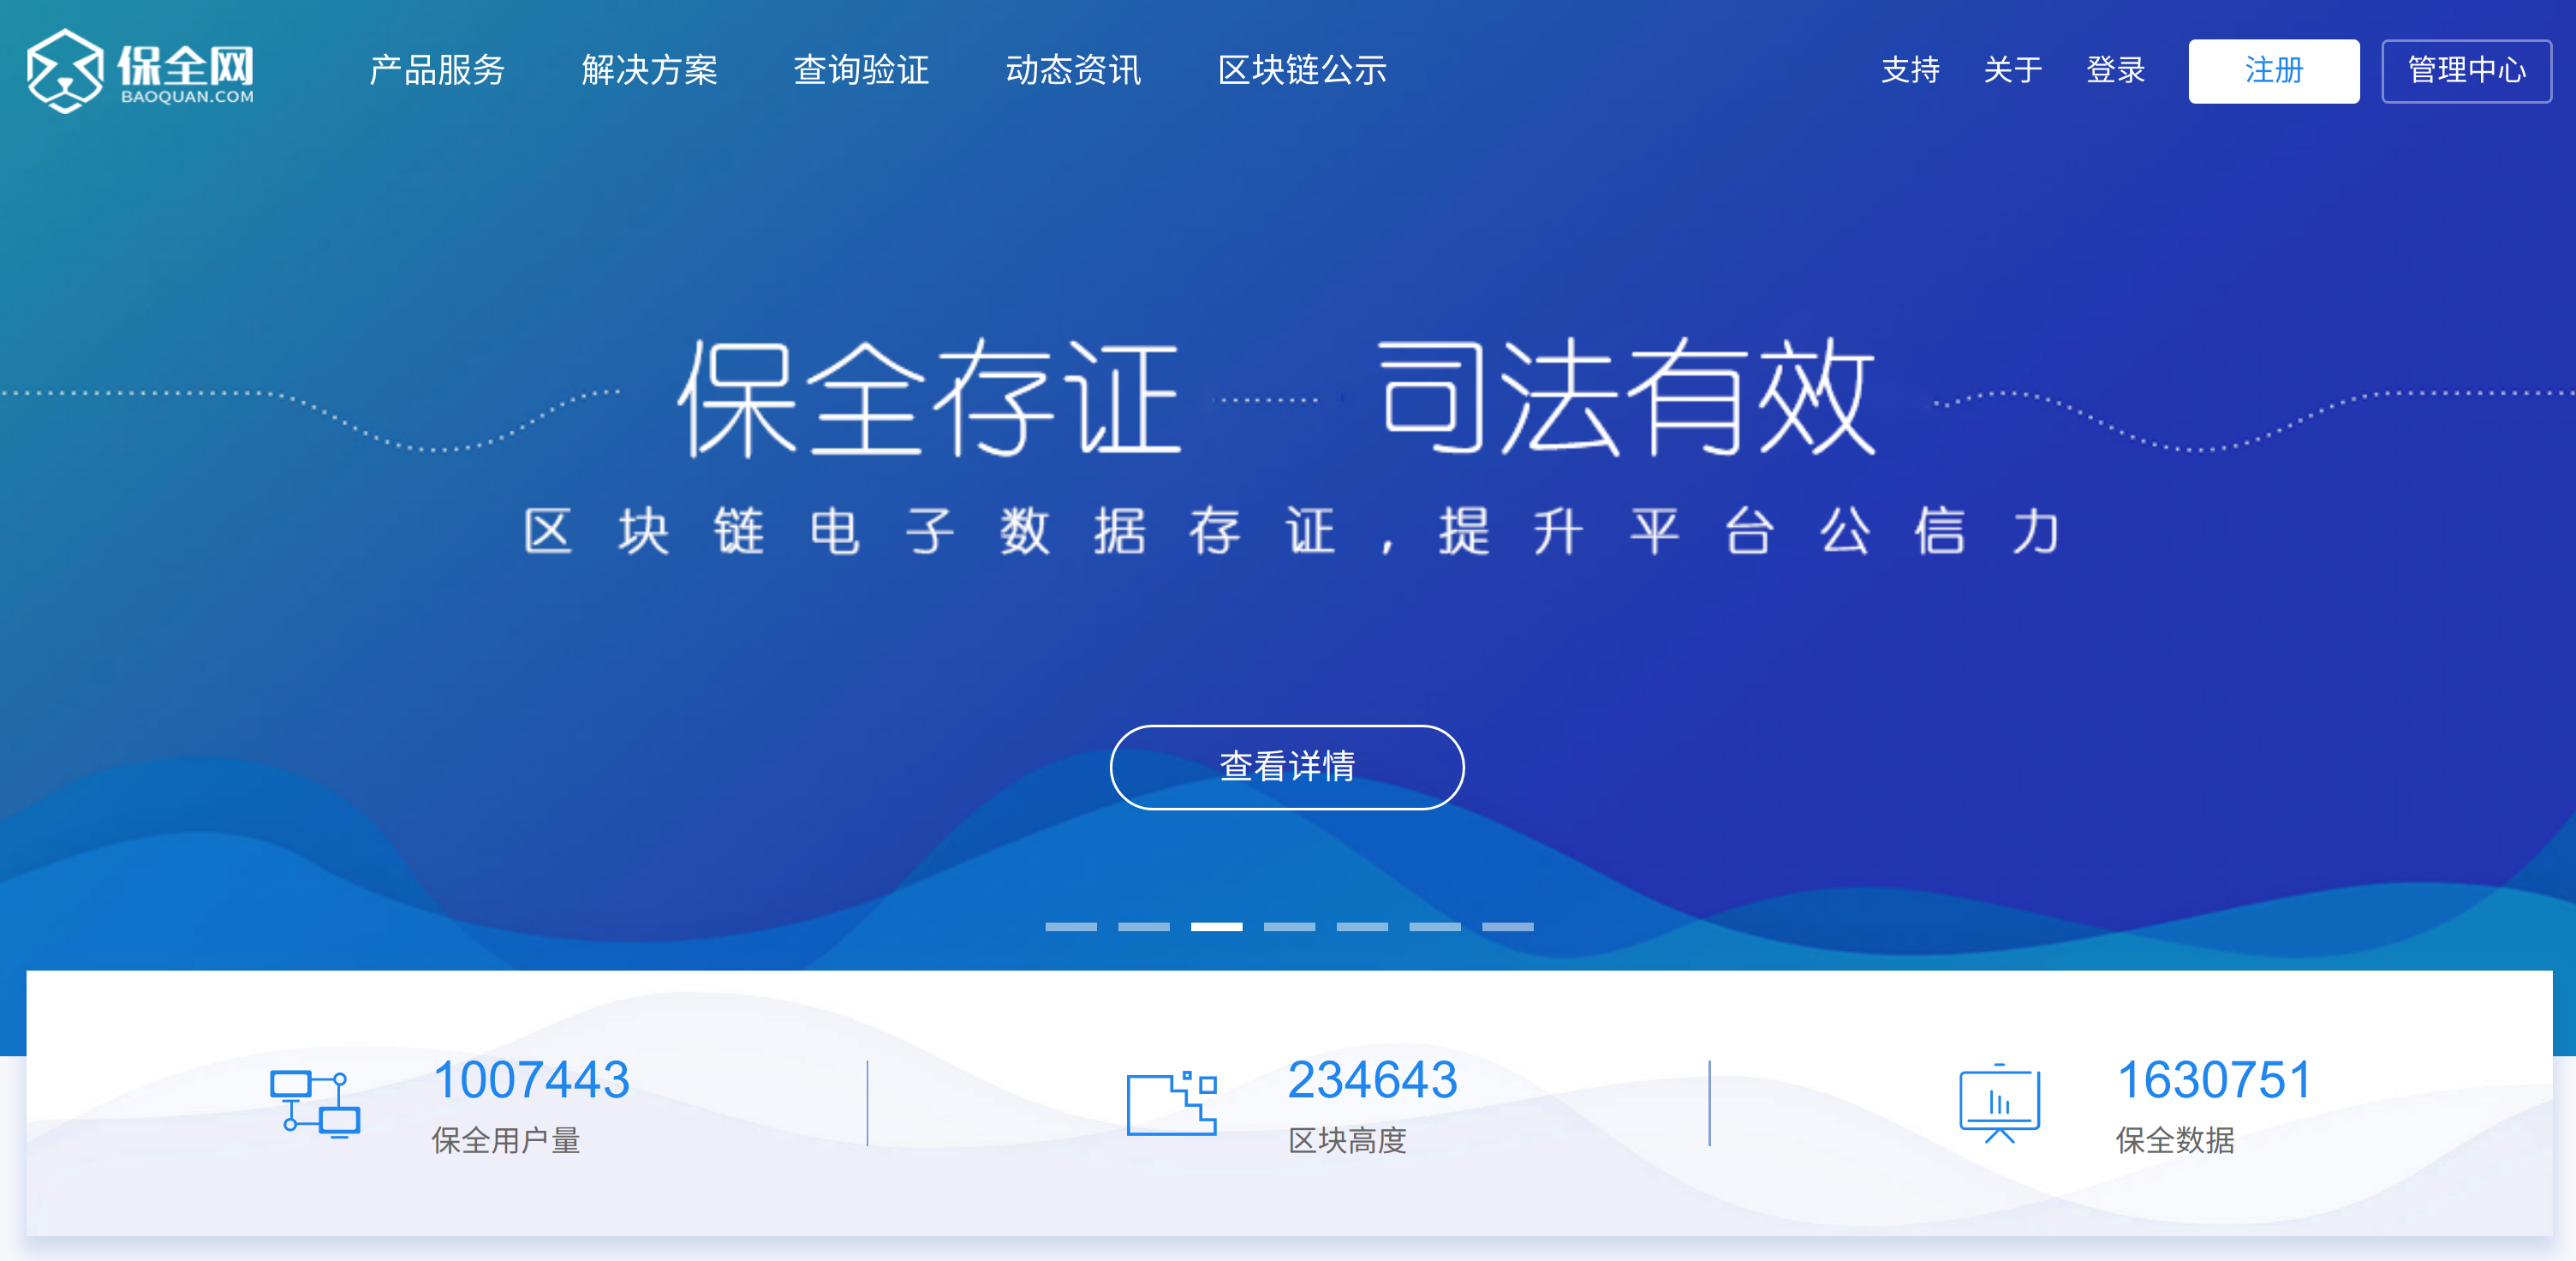
\includegraphics[width=11cm]{../pics/case_studies/baoquan}
		\caption{The Hangzhou Internet Court accepted evidence from the Baoquan Blockchain on a copyright case (\cite{chinesecourt2018})}
	\end{figure}
\end{frame}

\frame{
	\frametitle{Developer-friendly marketplace: The Bounties Network}
	\framesubtitle{Why not getting paid for your work?}
	\begin{figure}
		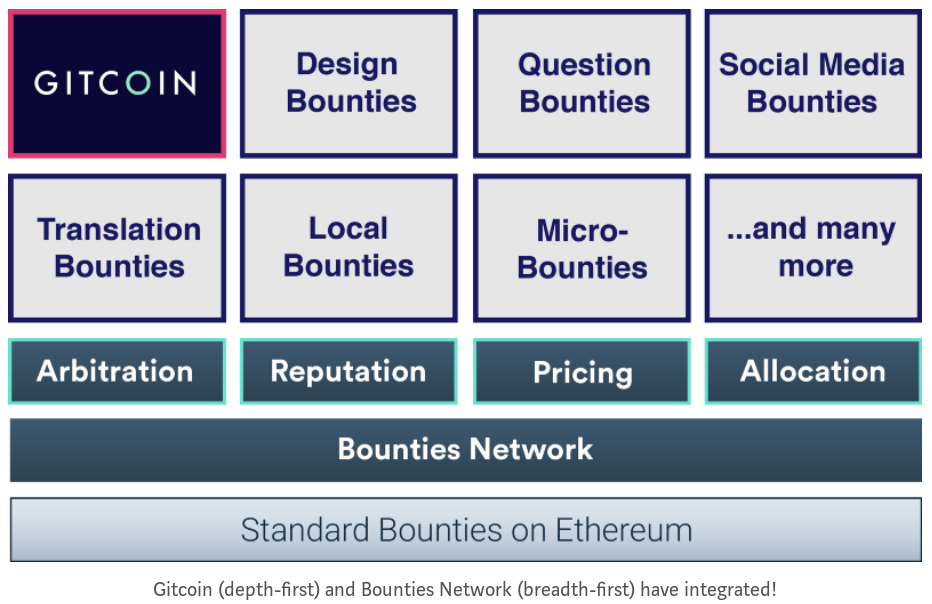
\includegraphics[width=11cm]{../pics/ConsenSys/bounties_network_stack}
		\framesubtitle{\url{https://bounties.network}}
	\end{figure}
}

\frame{
	\frametitle{Gitcoin}
	\framesubtitle{Gitcoin is not a coin}
	\begin{figure}
		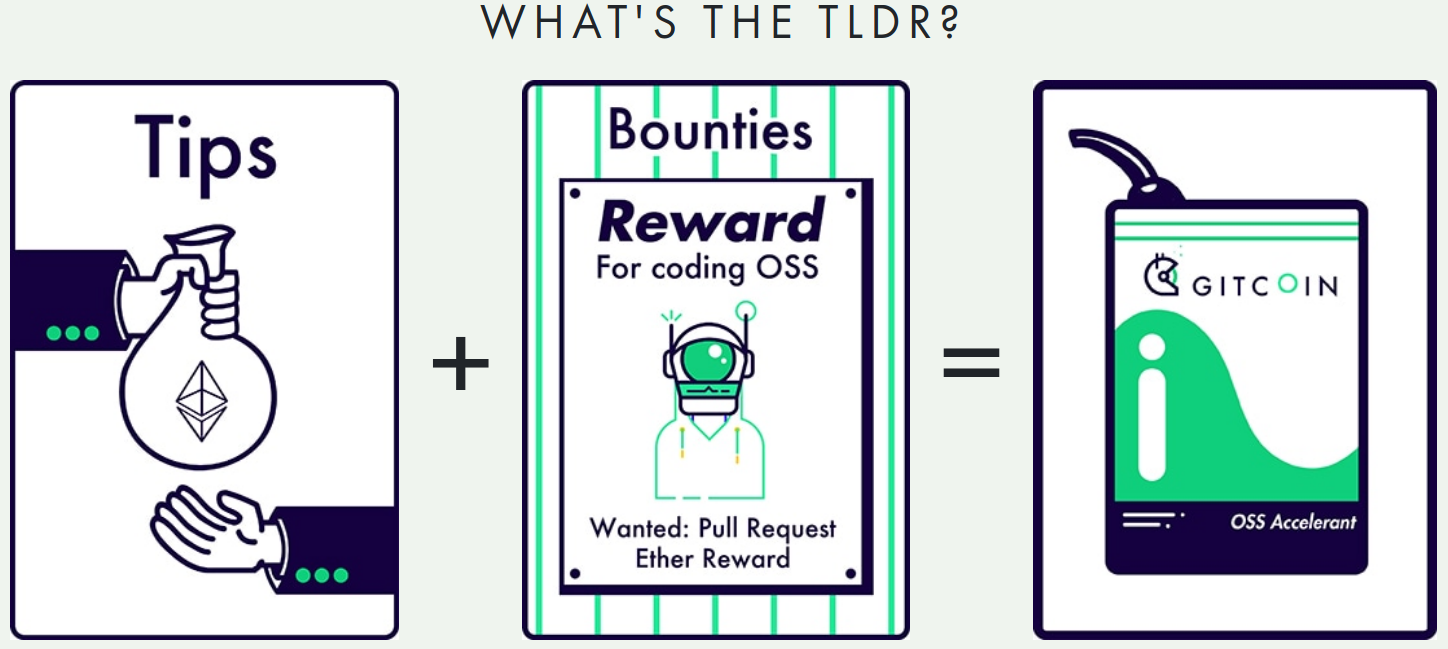
\includegraphics[width=11cm]{../pics/ConsenSys/gitcoin-tldr}
		\caption{\url{https://gitcoin.co}}
	\end{figure}
}







